% !TEX TS-program = pdflatex
% !TEX encoding = UTF-8 Unicode
\documentclass[11pt]{article} % use larger type; default would be 10pt

%%% PAGE DIMENSIONS
\usepackage{geometry}
\geometry{a4paper}

\usepackage{graphicx}
\graphicspath{ {img/} }

%%% PACKAGES
\usepackage[utf8]{inputenc}
\usepackage{cmap}
\usepackage[T2A]{fontenc}
\usepackage{booktabs} % for much better looking tables
\usepackage{array} % for better arrays (eg matrices) in maths
\usepackage{paralist} % very flexible & customisable lists (eg. enumerate/itemize, etc.)
\usepackage{verbatim}
\usepackage{subfig}
\usepackage[english,russian]{babel}
\usepackage{amssymb,latexsym,amsmath,amscd}

%%% HEADERS & FOOTERS
\usepackage{fancyhdr}
\pagestyle{fancy}
\renewcommand{\headrulewidth}{0pt}
\lhead{}\chead{}\rhead{}
\lfoot{}\cfoot{\thepage}\rfoot{}

%%% SECTION TITLE APPEARANCE
\usepackage{sectsty}
\allsectionsfont{\sffamily\mdseries\upshape}

%%% ToC (table of contents) APPEARANCE
\usepackage[nottoc,notlof,notlot]{tocbibind}
\usepackage[titles,subfigure]{tocloft}
\renewcommand{\cftsecfont}{\rmfamily\mdseries\upshape}
\renewcommand{\cftsecpagefont}{\rmfamily\mdseries\upshape}

% FIX: 'babel' with Russian option already defines \tg. 
% We check if it exists; if not, we define it. If yes, we leave it be.

\begin{document}
	
	%%% TITLE PAGE
	\title{ФЕДЕРАЛЬНОЕ ГОСУДАРСТВЕННОЕ БЮДЖЕТНОЕ
		ОБРАЗОВАТЕЛЬНОЕ УЧРЕЖДЕНИЕ ВЫСШЕГО ОБРАЗОВАНИЯ
		«МОСКОВСКИЙ ГОСУДАРСТВЕННЫЙ УНИВЕРСИТЕТ имени М.В. ЛОМОНОСОВА» ФИЗИЧЕСКИЙ ФАКУЛЬТЕТ КАФЕДРА МАТЕМАТИЧЕСКОГО МОДЕЛИРОВАНИЯ И ИНФОРМАТИКИ\\
		\vspace{30mm}
		КУРСОВАЯ РАБОТА\\
		Определение нижнего уровня облаков на основе информации стереосистемы.\vspace{15mm}}
	
	\author{
		\hspace{70mm}Выполнил: Устимов Иван Андреевич 535 гр.\\
		\vspace{15mm}
		\hspace{70mm}Научный руководитель: Чуличков Алексей Иванович\\
		\vspace{15mm}}
	
	\date{ Москва \\Май 2025}
	
	\maketitle
	\thispagestyle{empty}
	\pagebreak
	
	%%% OGLAVLENIE
	\tableofcontents
	\pagebreak
	
	%%% CONTENT
	
	\section{Обзор литературы}
	\vspace{3mm}\hspace{5mm}
	
	На сегодняшний день основным способом определения уровня облаков является
	использование облакомеров - приборов, в основе которых лежит измерение задержки отраженного лазерного сигнала от молекул, находящихся в облаках. Это достаточно надеждый метод, однако он требует наличия специального прибора и может
	быть применен лишь для некоторого диапазона высот. \par
	Альтернативой являются методы компьютерного зрения. На сегодняшний день
	придумано немало методов определения расстояний до объектов на основе как одного, так и нескольких снимков, в том числе нейросетевых [1]. В данной работе будет
	рассмотрен метод на основе стереопары, то есть двух снимков одной и той же сцены.\par
	Как правило, для нахождения расстояния до некоторой точки на изображении
	требуется информация о взаимном расположении камер между собой и информация
	об их внутренних параметрах. Для этого производят калибровку стереосистемы. На
	вход алгоритму калибровки подаются размеченные пары точек некоторого объекта
	с заранее известной геометрией (то есть мы можем восстановить в некоторой локальной системе координат объекта его точки в реальном масштабе), а на выходе
	получается матрица внутренних параметров, содержащая расстояния между камерами и матрцу поворота их системы координат, и матрица внутренних параметров,
	содержащая информацию о фокусных расстояниях камеры[4].\par
	В случае с съемкой облаков возникает некоторая проблема: ввиду того, что обе
	камеры, как правило, направлены в зенит, съемка калибровочного объекта, видимого на обеих камерах, затруднительна. Поэтому возникает необходимость в альтернативном способе калибровки.\par
	В работах [2,3] такой метод реализован: в качестве калибровочных объектов использовано солнце, а вместо матрицы внутренних и внешних параметров находится
	матрица перехода от пикселей первой картинки к пикселям второй (также называемая гомографией или аффинным преобразованием).
	
	\pagebreak
	
	\section{Геометрическая модель эксперимента}
	\vspace{3mm}\hspace{5mm}
	
	Для оценки расстояния до объекта по стереопаре его изображений опишем сначала математическую модель стереопары изображений при условии, что обе фотокамеры имеют одни и те же параметры (увеличение) и технические характеристики,
	а их оптические оси направлены в зенит.\par
	С каждой фотокамерой свяжем декартову систему координат, в которой ось $OiZ$
	направлена вертикально вверх и совпадает с ее оптической осью, горизонтальная ось
	$OiX$ проходит через центры камеры и направлена от камеры $SL$ к камере $SR$. Пусть
	облако расположено на высоте $D$, расстояние между фотокамерами по горизонтальной оси равно $B$ (размер базы). Пусть $x_0$ - горизонтальный размер пространственной
	области на высоте $D$, изображаемой фотокамерой, $\phi_0$ - угол обзора камеры (Рис. 1).
	Тогда
	\begin{equation}
		D = \frac{x_0}{2\tg(\phi_0/2)}
	\end{equation}
	
	\begin{figure}[h!]
		\center
		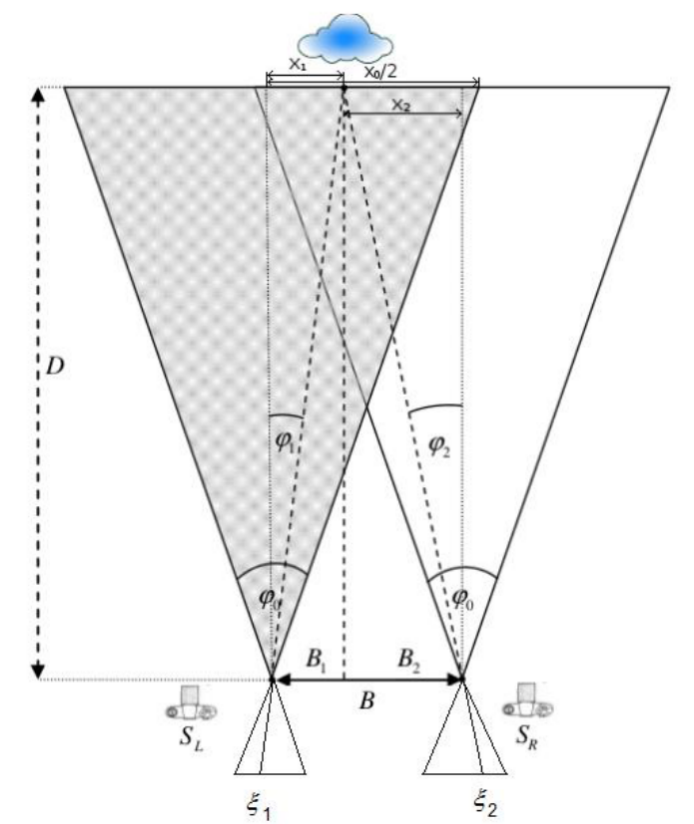
\includegraphics[scale=0.5]{geom_model}
		\caption{Геометрическая модель стереопары}
	\end{figure}
	
	Выберем точку облака (для наглядности на Рис. 1 эта точка лежит в плоскости,
	проходящей через оптические оси обеих камер). Обозначим $x_1$ и $x_2$ координаты выбранной точки облака вдоль осей $O1X$ и $O2X$ в системе координат первой и второй
	камер соответственно. Для точки облака, расположенной в плоскости оптических
	осей, выполнено равенство $|x_1 - x_2| = B$. Поэтому вместо (1) имеем:
	
	\begin{equation}
		D = \frac{Bx_0}{2\tg(\phi_0/2)|x_1 - x_2|}
	\end{equation}
	
	В формуле (2) наблюдаемыми являются параметры $B$ (стереобаза), $\phi_0$ (угол обзора фотокамеры) и отношение $\frac{x_0}{|x_1 - x_2|}$
	- оно равно отношению $\frac{\xi_0}{|\xi_1 - \xi_2|}$
	размера кадра $\xi_0$ к модулю разности координат изображений выбранной точки облака на первом и
	втором кадре $|\xi_1 - \xi_2|$. Итак, формула для вычисления высоты облака есть:
	
	\begin{equation}
		D = \frac{B\xi_0}{2\tg(\phi_0/2)|\xi_1 - \xi_2|}
	\end{equation}
	
	\subsection{Погрешность расстояния}
	\vspace{3mm}\hspace{5mm}
	
	Погрешность определения высоты облака с помощью формулы (3) оценим по
	формуле для погрешности косвенных измерений:
	
	\[
	\Delta D = \sqrt{\left(\frac{\partial D}{\partial B} \Delta B\right)^2 + \left(\frac{\partial D}{\partial \phi_0} \Delta \phi_0\right)^2 + \left(\frac{\partial D}{\partial \xi_1} \Delta \xi_1\right)^2 + \left(\frac{\partial D}{\partial \xi_2} \Delta \xi_2\right)^2}
	\]
	
	Заметим, что $\Delta\xi_0 = 0$, т.к. размер кадра мы всегда знаем точно. Также,
	обычно $\Delta\xi_1 = \Delta\xi_2$, поэтому формула упрощается:
	
	\[
	\Delta D = \sqrt{\left(\frac{\partial D}{\partial B} \Delta B\right)^2 + \left(\frac{\partial D}{\partial \phi_0} \Delta \phi_0\right)^2 + 2\left(\frac{\partial D}{\partial \xi_1} \Delta \xi_1\right)^2}
	\]
	
	Если проанализировать, какие слагаемые дают наибольший вклад в погрешность, то заметим, что подавляющую часть вносят погрешности: 
	\[
	\Delta D \approx \sqrt{ \left( \frac{\partial D}{\partial \xi_1} \Delta \xi_1 \right)^2 + \left( \frac{\partial D}{\partial \xi_2} \Delta \xi_2 \right)^2}
	\]
	Существенно уменьшить эти погрешности можно:
	\begin{enumerate}
		\item увеличивая размер кадра;
		\item повышая точность определения координат $\xi_i$ («субпиксельная точность»).
	\end{enumerate}
	И то и другое приведет к росту числа вычислений. В данной работе для сокращения вычислительных затрат рассматриваются следующие два подхода:
	\begin{enumerate}
		\item деление спектра Grayscale-изображения (яркость 0 . . . 255) на $< 256$ промежутков, соответствующих новым (средним по промежутку) яркостям;
		\item Применение кластеризации для векторов смещений, с целью отсева шумовых точек.
	\end{enumerate}
	
	\pagebreak
	
\section{Определение аффинного преобразования}
\vspace{3mm}\hspace{5mm}

\textbf{Неформальная постановка.} Стереосистема состоит из двух камер, выдающих изображения №1 и №2. Для применения формулы (3) необходимо, чтобы плоскости осей камер совпадали, что на практике недостижимо. Требуется найти такое проекционное преобразование, которое компенсирует взаимный поворот и сдвиг камер, приводя изображения к виду, эквивалентному параллельным оптическим осям.

\textbf{Формальная постановка.} Пусть заданы два изображения --- №1 (от камеры $SL$) и №2 (от камеры $SR$). Требуется определить матрицу аффинного преобразования $H \in \mathbb{R}^{3 \times 3}$ вида
\[
H = \begin{pmatrix} r_1 & r_2 & t_1 \\ r_3 & r_4 & t_2 \\ 0 & 0 & 1 \end{pmatrix},
\]
где подматрица $\begin{pmatrix} r_1 & r_2 \\ r_3 & r_4 \end{pmatrix}$ образует матрицу поворота системы координат, а $(t_1, t_2)^\top$ --- вектор сдвига. Калибровка производится по набору из $K$ пар соответствующих точек $(x^{(i)}_1, y^{(i)}_1)$ на изображении №1 и $(x^{(i)}_2, y^{(i)}_2)$ на изображении №2, $i = 1, \dots, K$, таких, что при совмещённых осях каждая точка переходит сама в себя. Матрица $H$ ищется из условия минимума невязки:
\[
\sum_{i=1}^{K} \left\| \begin{pmatrix} x^{(i)}_1 \\ y^{(i)}_1 \\ 1 \end{pmatrix} - H \begin{pmatrix} x^{(i)}_2 \\ y^{(i)}_2 \\ 1 \end{pmatrix} \right\|^2 \to \min.
\]
Система разрешима при $K \ge 3$ парах точек общего положения.

В дальнейшем, для ясности изложения, введём обозначения: изображение №1 --- снимок, к которому применяется аффинное преобразование $H$, а изображение №1' --- результат его применения, то есть $I_{1'} = \mathcal{W}_H(I_1)$, где $\mathcal{W}_H$ --- оператор аффинного преобразования. Изображение №2 остаётся неизменным. Смещение $\Delta\xi$ определяется уже между преобразованным изображением №1' и исходным изображением №2.

В контексте поставленной задачи, встаёт вопрос: как находить соответствия между изображениями для калибровки $H$? Сами по себе облака обладают достаточно однородной структурой, и определение точных соответствий затруднительно. Тем не менее, соответствия легко находить по солнцу: это бесконечно удалённый объект, который на обеих камерах при должной калибровке будет проецироваться в одни и те же координаты на обоих снимках. Таким образом, находится такое преобразование $H$, что бесконечно удалённые объекты не меняют своего положения в плоскости изображения. То есть, с учётом направления осей камер, это означает совмещение их плоскостей, что позволяет применять формулу (3).
	
	\pagebreak
	
\section{Определение смещения между изображениями}
\vspace{3mm}\hspace{5mm}

Задача определения смещения между кадрами состоит в нахождении вектора смещения $\Delta\vec r = (\Delta\xi, \Delta\eta)$ на плоскости изображения, соединяющего точку на преобразованном изображении №1' с соответствующей точкой на изображении №2: $\Delta\vec r = (x_{1'}, y_{1'}) - (x_2, y_2)$. В контексте формулы (3) интерес представляет лишь горизонтальная компонента $\Delta\xi = x_{1'} - x_2$ (называемая диспарантностью или параллаксом); вертикальная компонента $\Delta\eta$ после аффинного преобразования должна быть близка к нулю в силу выравнивания оптических осей. В компьютерном зрении задача поиска соответствий известна как \textit{feature matching} (сопоставление ключевых точек, рис. 2) [11], а выделение информативных точек и построение их описаний --- как \textit{feature extraction} (детектирование и описание ключевых точек) [11].

\begin{figure}[h!]
	\center
	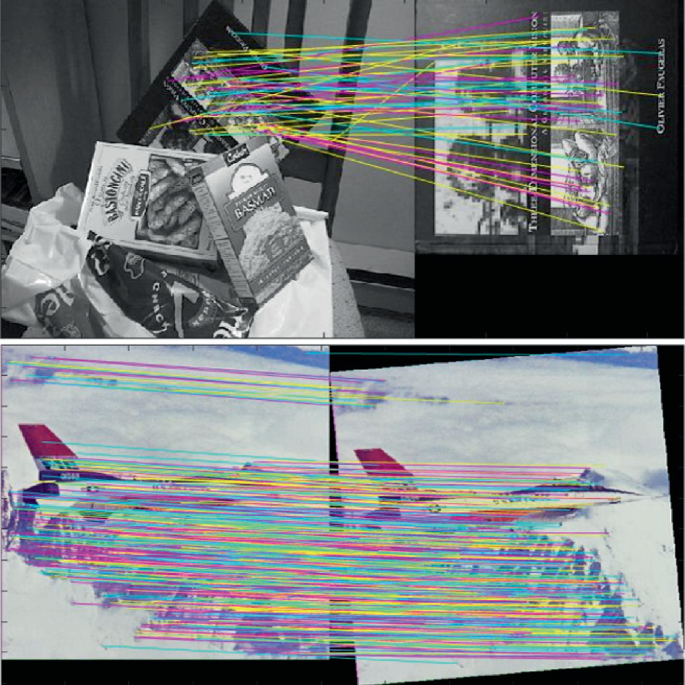
\includegraphics[scale=0.5]{matching}
	\caption{Feature matching}
\end{figure}

Задача \textit{feature extraction} состоит в выявлении наиболее информативных точек
картинки и создании дескрипторов данных точек. Дескриптор --- это вектор, содержащий информацию о локальном окружении данной точки. Разные алгоритмы по
разному формируют дескрипторы. Например, детекторы на основе SIFT в качестве
дескрипторов используют гистограмму градиентов локального окружения точки.
Для классических подходов вычисление информативных точек необходимо для
поиска соответствий, однако нейросети могут вычислять соответствия напрямую по
паре изображений.\par
В данной работе для выделения соответствий использовалась предобученная нейросеть
LOFTR [6] --- метод, не требующий отдельного этапа детектирования ключевых точек (detector-free). Особенность данной нейросети в том, что она обучалась предсказывать соответствия между точками напрямую по двум изображениям. Притом эти
предсказания плотные --- то есть модель способна генерировать соответствия на небольшом
расстоянии друг от друга. В архитектуре применяется техника ViT (Vision Transformer) [7] --- каждый
небольшой патч изображения кодируется энкодером в эмбеддинг с помощью свёрточной нейросети, а затем к этим эмбеддингам применяются attention-слои. Таким
образом, в отличие от стандартных свёрточных энкодеров, поле восприятия нейросети охватывает всё изображение, и она способна выучивать взаимодействия между
удалёнными частями изображения. Подробнее про архитектуру можно прочитать в
статье [6].
	
	\pagebreak
	
	\section{Практическая часть}
\subsection{Поиск афинного преобразования}
\vspace{3mm}\hspace{5mm}

Поиск аффинного преобразования $H$ производится с помощью библиотеки OpenCV
функцией \texttt{cv2.estimateAffine2D()}, на вход которой подаются два массива точек — на изображении №1 и на изображении №2 соответственно. Начальное приближение задаётся с помощью
алгоритма RANSAC. Затем это приближение уточняется за счёт численной аппроксимации матрицы аффинного преобразования.\par
В проведённом эксперименте использовались соответствия по положению солнца на изображениях №1 и №2. Как показала практика, брать большее число точек для калибровки (например, дополнительные точки на облаках) не имеет смысла, так
как они будут отсеяны алгоритмом RANSAC как не удовлетворяющие модели жёсткого преобразования. Калибровка на основе снимков от 29 мая 2023 года дала следующую матрицу аффинного преобразования:

\begin{equation}
	H = \begin{pmatrix} 0.9954\ 0.0424 \ 129 \\ -0.0202 \ 0.9810 \ -28 \\0 \ 0 \ 1 \end{pmatrix}
\end{equation}

Можно заметить, что матрица поворота системы координат близка к единичной, что говорит о несильном повороте камер друг относительно друга. Это также
согласуется с результатами из предыдущих работ [2,3].

\subsection{Определение нижней границы облачности}
\vspace{3mm}\hspace{5mm}

Экспериментальные данные представляют собой серии парных снимков облачного неба, полученных стереосистемой в дневное время в период с мая по июль 2023 года. Снимки делались с интервалом $\approx 10$ с; для каждого момента времени имеется два кадра — от камеры $SL$ (изображение №1) и от камеры $SR$ (изображение №2). Размер каждого кадра составляет $1920 \times 1080$ пикселей; для анализа использовалась центральная область размером $640 \times 640$ пикселей, вырезаемая из каждого снимка.

Обработка каждой стереопары выполняется в следующем порядке. Сначала изображение №1 подвергается аффинному преобразованию $H$, полученному на этапе калибровки, — результат обозначается как изображение №1'. Затем нейросеть LOFTR находит соответствия между изображением №1' и (неизменённым) изображением №2 (рис. 3).

\begin{figure}[h!]
	\center
	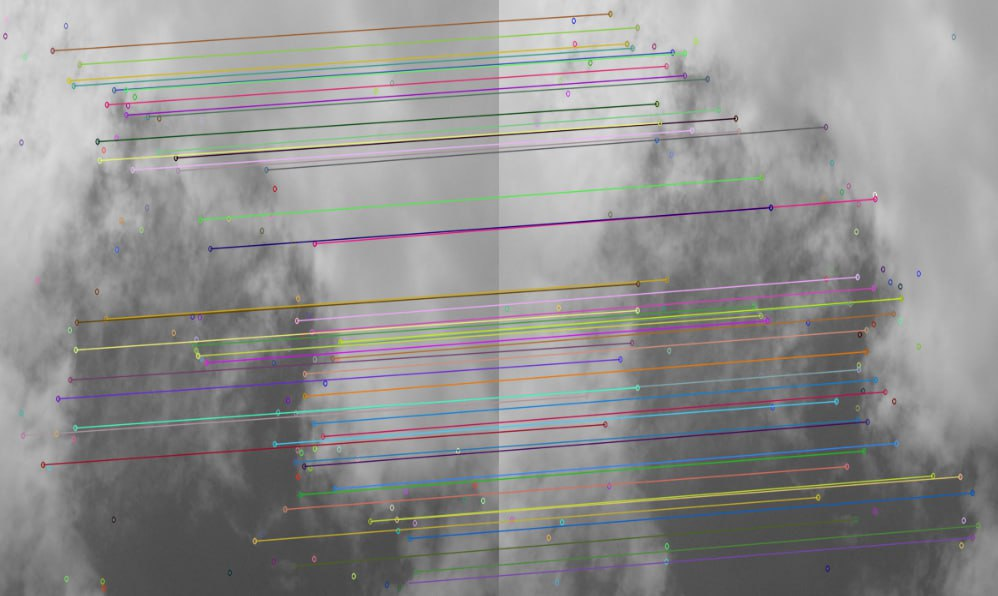
\includegraphics[scale=0.5]{clouds}
	\caption{Результат работы LOFTR: соответствия между изображением №1' (после аффинного преобразования) и изображением №2 (исходным)}
\end{figure}

Из полученных пар соответствий вычисляются векторы смещений $\Delta\vec r = (x_{1'}, y_{1'}) - (x_2, y_2)$ простым векторным вычитанием. Таким образом, аффинное преобразование применяется до поиска соответствий, а не после — это исключает необходимость отдельного этапа преобразования координат найденных точек.\par
Для оценки высоты нижней границы облачности (НГО) можно было бы использовать среднее смещение по всем найденным соответствиям. Однако ввиду неидеальности алгоритма LOFTR часть соответствий оказывается ошибочной (ложные мэтчи), что приводит к появлению выбросов в наборе векторов смещений. С целью обработки выбросов и группировки валидных векторов смещений, в работе использована иерархическая кластеризация, а
именно алгоритм HDBSCAN (результат кластеризации на рис. 4, распределение высот,
полученное по параллаксам из этих же кластеров на рис. 6).
	
	\begin{figure}[h!]
		\center
		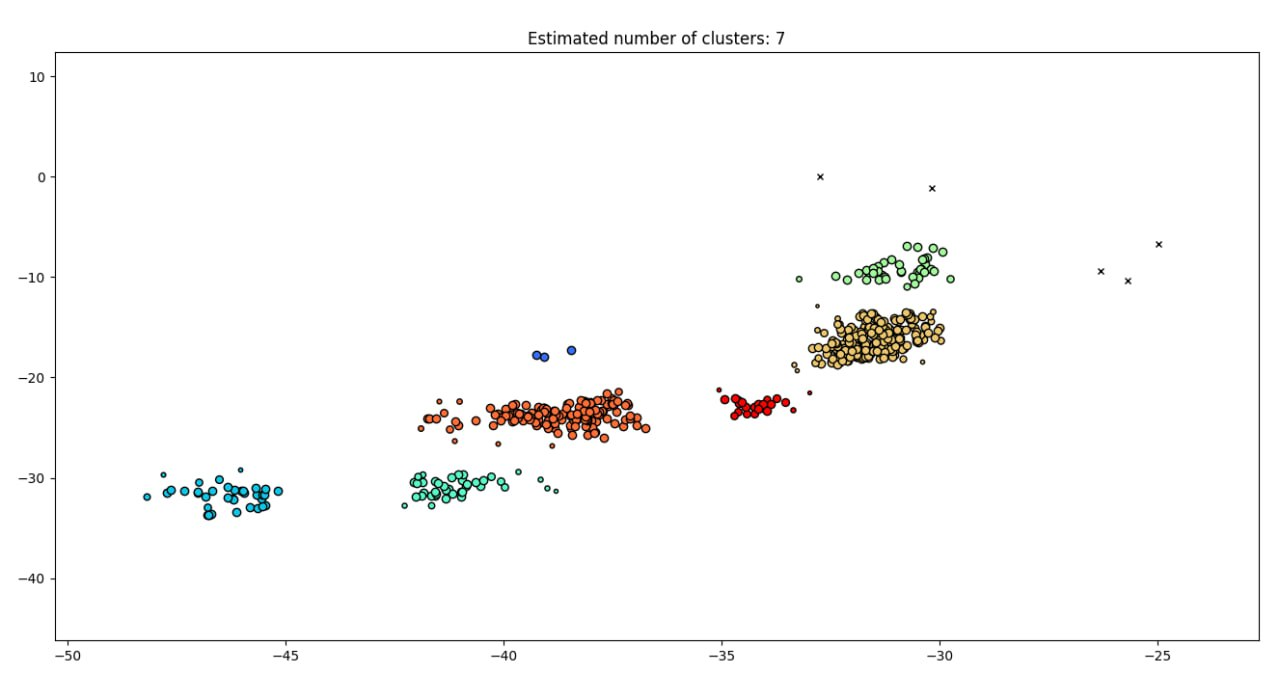
\includegraphics[scale=0.5]{cluster} % Name inferred
		\caption{Кластеризация в пространстве векторов смещений (px)}
	\end{figure}
	
	\begin{figure}[h!]
		\center
		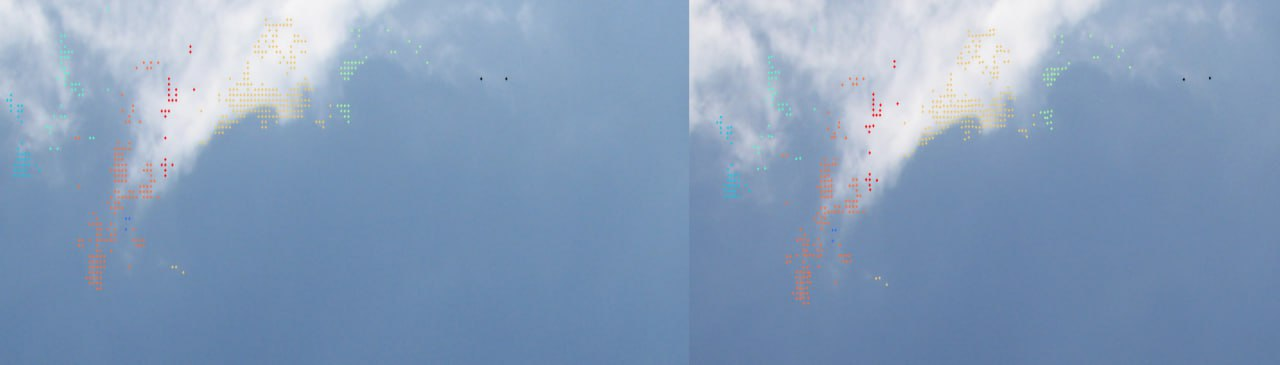
\includegraphics[scale=0.5]{localization} % Name inferred
		\caption{Локализация соответствий на исходных изображениях}
	\end{figure}
	
	Кластеризация также помогает отчасти решить проблему неодноротности нижней границы. Дело в том, что облака имеют неоднородную по нижнему уровню
	высоты структуру. На фотографиях, как правило, присутствуют такие неоднородные участки, и соответственно смещение для таких участков оказывается разное.
	Поэтому в пространстве векторов смещения выделяются кластеры, соотносящиеся
	к разным высотам облаков. Кластеризация решает задачу о выделении таких кластеров, и в ряде случаев выделяется более одного значимого кластера (что в таблице~\ref{table:1} обозначено через знак <</>>, разделяющий два кластера, соответствующих двум разным высотным уровням облачности).

	Для верификации результатов в эксперименте использовался лазерный высотомер (ceilometer) --- прибор, измеряющий высоту нижней границы облачности по времени задержки отражённого лазерного импульса. Высотомер был расположен в непосредственной близости от стереосистемы, что позволило получить независимую эталонную оценку высоты для каждого временного среза.
	
	\begin{figure}[h!]
		\center
		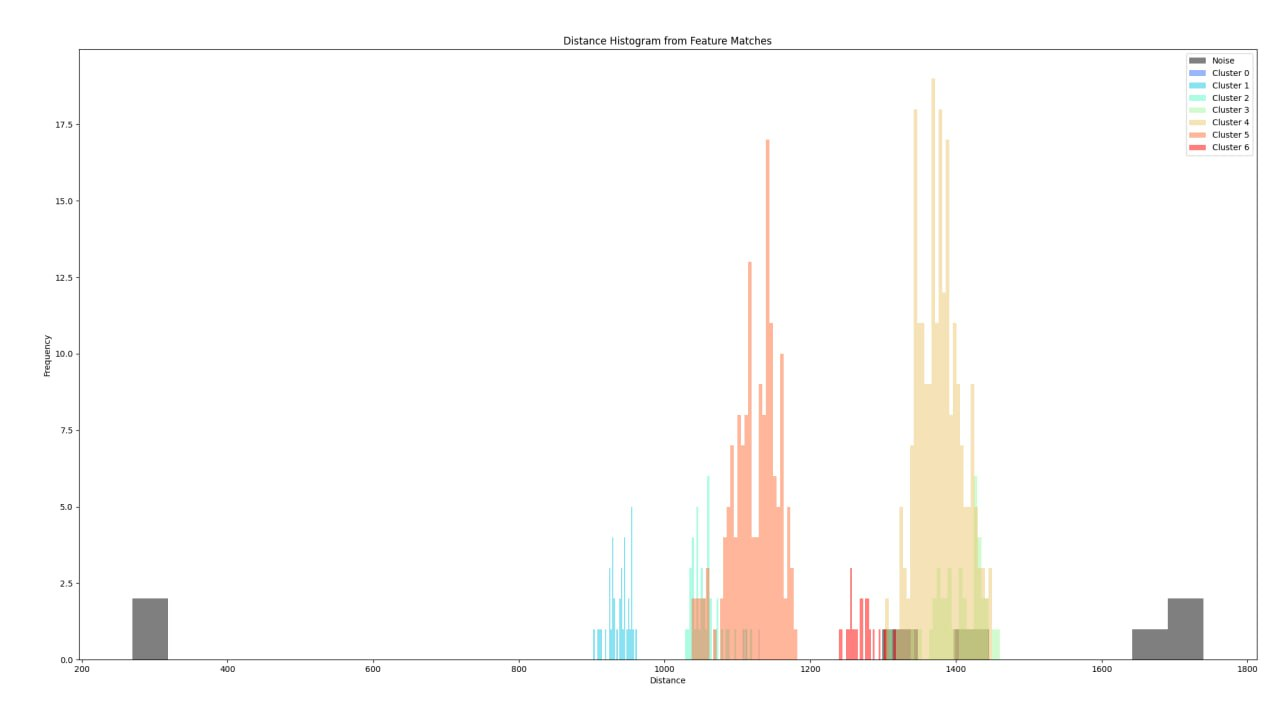
\includegraphics[scale=0.5]{height_dist}
		\caption{Распределение высот в рамках кластеров (м). Эталонная высота по данным высотомера --- 1300 м}
	\end{figure}
	
	Наблюдается, что локализация точек в пространстве векторов смещений коррелирует с локализацией соответствующих точек на изображении (рис.~4 и рис.~5). С физической точки зрения, такая корреляция ожидаема: участки облачности, имеющие близкую высоту (а следовательно, близкое смещение), часто образуют связные области в плоскости изображения. Однако обратное неверно: близкие в пространстве векторов смещений точки могут находиться в геометрически удалённых участках изображения, и наоборот --- получение двух идентичных векторов смещения сводится к простому линейному сдвигу точек соответствия на паре изображений.\par
	Для оценки погрешности смещения использовано стандартное отклонение векторов смещений в кластере, однако его не стоит интерпретировать исключительно как ошибку измерения.
	Ввиду описанной выше связи между кластеризацией по смещению и пространственной локализацией, можно утверждать, что в рамках одного
	кластера рассчитанные по каждому из соответствий высоты дают значения для
	участков облака, близко расположенных к центру кластера. Это означает, что погрешность также содержит естественный разброс высоты нижней границы облака, связанный с её неоднородностью. Впрочем, это вытекает и из распределения
	высот, рассчитанного по точкам из разных кластеров.\par
	Результаты определения высоты нижней границы облачности на основе полученных смещений
	приведены в таблице~\ref{table:1}:
	
	\begin{table}[h!]
		\centering
		\begin{tabular}{||c c c||} 
			\hline
			Оценка НГО алгоритмом (м) & Эталонная НГО (высотомер, м) & Дата снимков  \\ [0.5ex] 
			\hline\hline
			2381 $\pm$ 304 & 2570 & 2023.06.01; 17:42 \\
			2554 $\pm$ 210 & 2570 & 2023.06.01; 18:42 \\
			2081 $\pm$ 315 & 2090 & 2023.06.02; 13:42 \\
			2069/3230 $\pm$ 259/ 384 & 2350/3190 & 2023.06.02; 15:42 \\
			2090 $\pm$ 53 & 1810 & 2023.06.06; 15:17 \\
			2256 $\pm$ 346 & 2060 & 2023.06.20; 14:01 \\
			2483 $\pm$ 392 & 1850 & 2023.07.02; 18:45 \\
			3443 $\pm$ 738 & 1310 & 2023.05.21; 11:12 \\
			2510 $\pm$ 347 & 2430 & 2023.06.01; 16:41 \\ [1ex] 
			\hline
		\end{tabular}
		\caption{Высота нижней границы облачности (НГО): сравнение алгоритмической оценки с данными высотомера}
		\label{table:1}
	\end{table}
	
	Погрешность измерений --- стандартное отклонение координат точек в соответствующем кластере. Можно заметить, что для снимков, близких по дате друг к другу, точность алгоритмической оценки относительно высотомера наилучшая. Понижение точности для снимков, отстоящих по дате от калибровочного дня, скорее всего связано со случайным изменением относительного положения камер (например, вследствие температурных деформаций крепления или ветровых нагрузок). Дело в том, что
	погрешность в один пиксель способна дать погрешность в определении высоты в
	$\approx 30$ метров. При повторных калибровках матрицы аффинного преобразования, выполненных в разные дни, было замечено, что вектор смещения для одного и того же объекта мог отличаться на величину до 30 пикселей. Это говорит о необходимости регулярной калибровки стереосистемы --- желательно перед каждым сеансом наблюдений. Ниже будет рассмотрено, как
	зашумление калибровочной матрицы влияет на точность результата.
	
\subsection{Анализ чувствительности к погрешности матрицы поворота гомографии}
\vspace{3mm}\hspace{5mm}

Имеет смысл рассматривать лишь влияние погрешности матрицы поворота гомографии: погрешность вектора сдвига напрямую и очевидно влияет на результат. Изменение сдвига по оси
$y$ не влияет на вычисление высоты по построению (формула (3) зависит только от горизонтальной компоненты $|\xi_1 - \xi_2|$), а изменение сдвига по оси $x$
вызовет прямое изменение согласно формуле (3); его эффект оценён выше при анализе погрешности (1 пикс $\approx$ 30 м). Не так очевидно влияние погрешности матрицы поворота, содержащейся в
гомографии.\par
Для более детального исследования проведена серия экспериментов, в которых
к исходной матрице поворота гомографии последовательно добавлялось систематическое возмущение в виде дополнительного угла поворота $\theta$ в диапазоне от $0^\circ$ до $15^\circ$ с шагом $1.5^\circ$ (угол $\theta$ --- не случайная величина, а детерминированный параметр, перебираемый для оценки чувствительности метода). При этом остальные элементы гомографии оставались неизменными. Для каждого значения $\theta$ вычислялась итоговая
высота нижней границы облачности по той же методике, что и в основном эксперименте.

\begin{figure}[h!]
	\center
	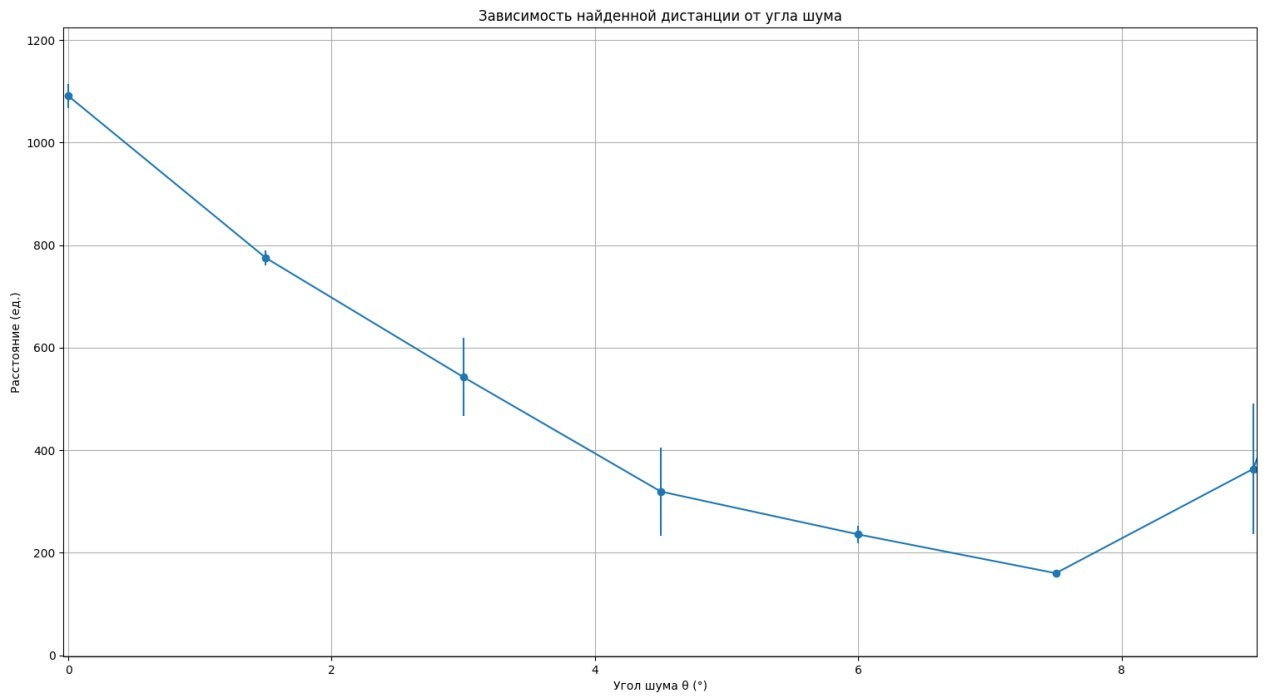
\includegraphics[scale=0.25]{ablation}
	\caption{Зависимость оценки высоты нижней границы облачности (м) от величины дополнительного угла поворота $\theta$ (градусы) в матрице гомографии. Эталонная высота по данным высотомера --- 1050 м (данные от 25 мая 2023 г., не входящие в таблицу~\ref{table:1}).}
\end{figure}

Как показано на рис.~7, зависимость ошибки оценки высоты от величины углового возмущения имеет выраженный нелинейный характер. Уже при $\theta \approx 1.5^\circ$ отклонение от эталонной высоты превышает 200 м, а при $\theta \ge 2^\circ$ оценки расходятся более чем
на 400 м.\par
Такой сильный эффект объясняется малым параллаксом для данной стереосистемы: при высоте облачности $\approx 1000$ м и базе $\approx 1$ м горизонтальное смещение между изображениями составляет порядка нескольких десятков пикселей. Поэтому
достаточно малого поворота изображений друг относительно друга, чтобы вызвать существенную ошибку в оценке смещения, а следовательно --- и в оценке высоты (1 пикс $\approx$ 30 м, что следует из формулы (3) при подстановке параметров данной стереосистемы).
	
\section{Анализ временных рядов}
\vspace{3mm}\hspace{5mm}

Для верификации работы стереосистемы проведён сравнительный анализ временных рядов высоты нижней границы облачности (НГО), полученных разработанным алгоритмом и с помощью высотомера ДОЛ-2. Съёмка изображений производилась 25 мая 2023 года в дневное время. Параллельно со съёмкой выполнялось измерение НГО высотомером, расположенным в непосредственной близости от стереосистемы. Это позволило получить эталонный временной ряд высоты $H_{\text{ref}}$ для сравнения с данными стереосистемы $H_{\text{stereo}}$. Для анализа использовалась центральная область каждого кадра размером $640 \times 640$ пикселей.
	
	\begin{figure}[h!]
		\center
		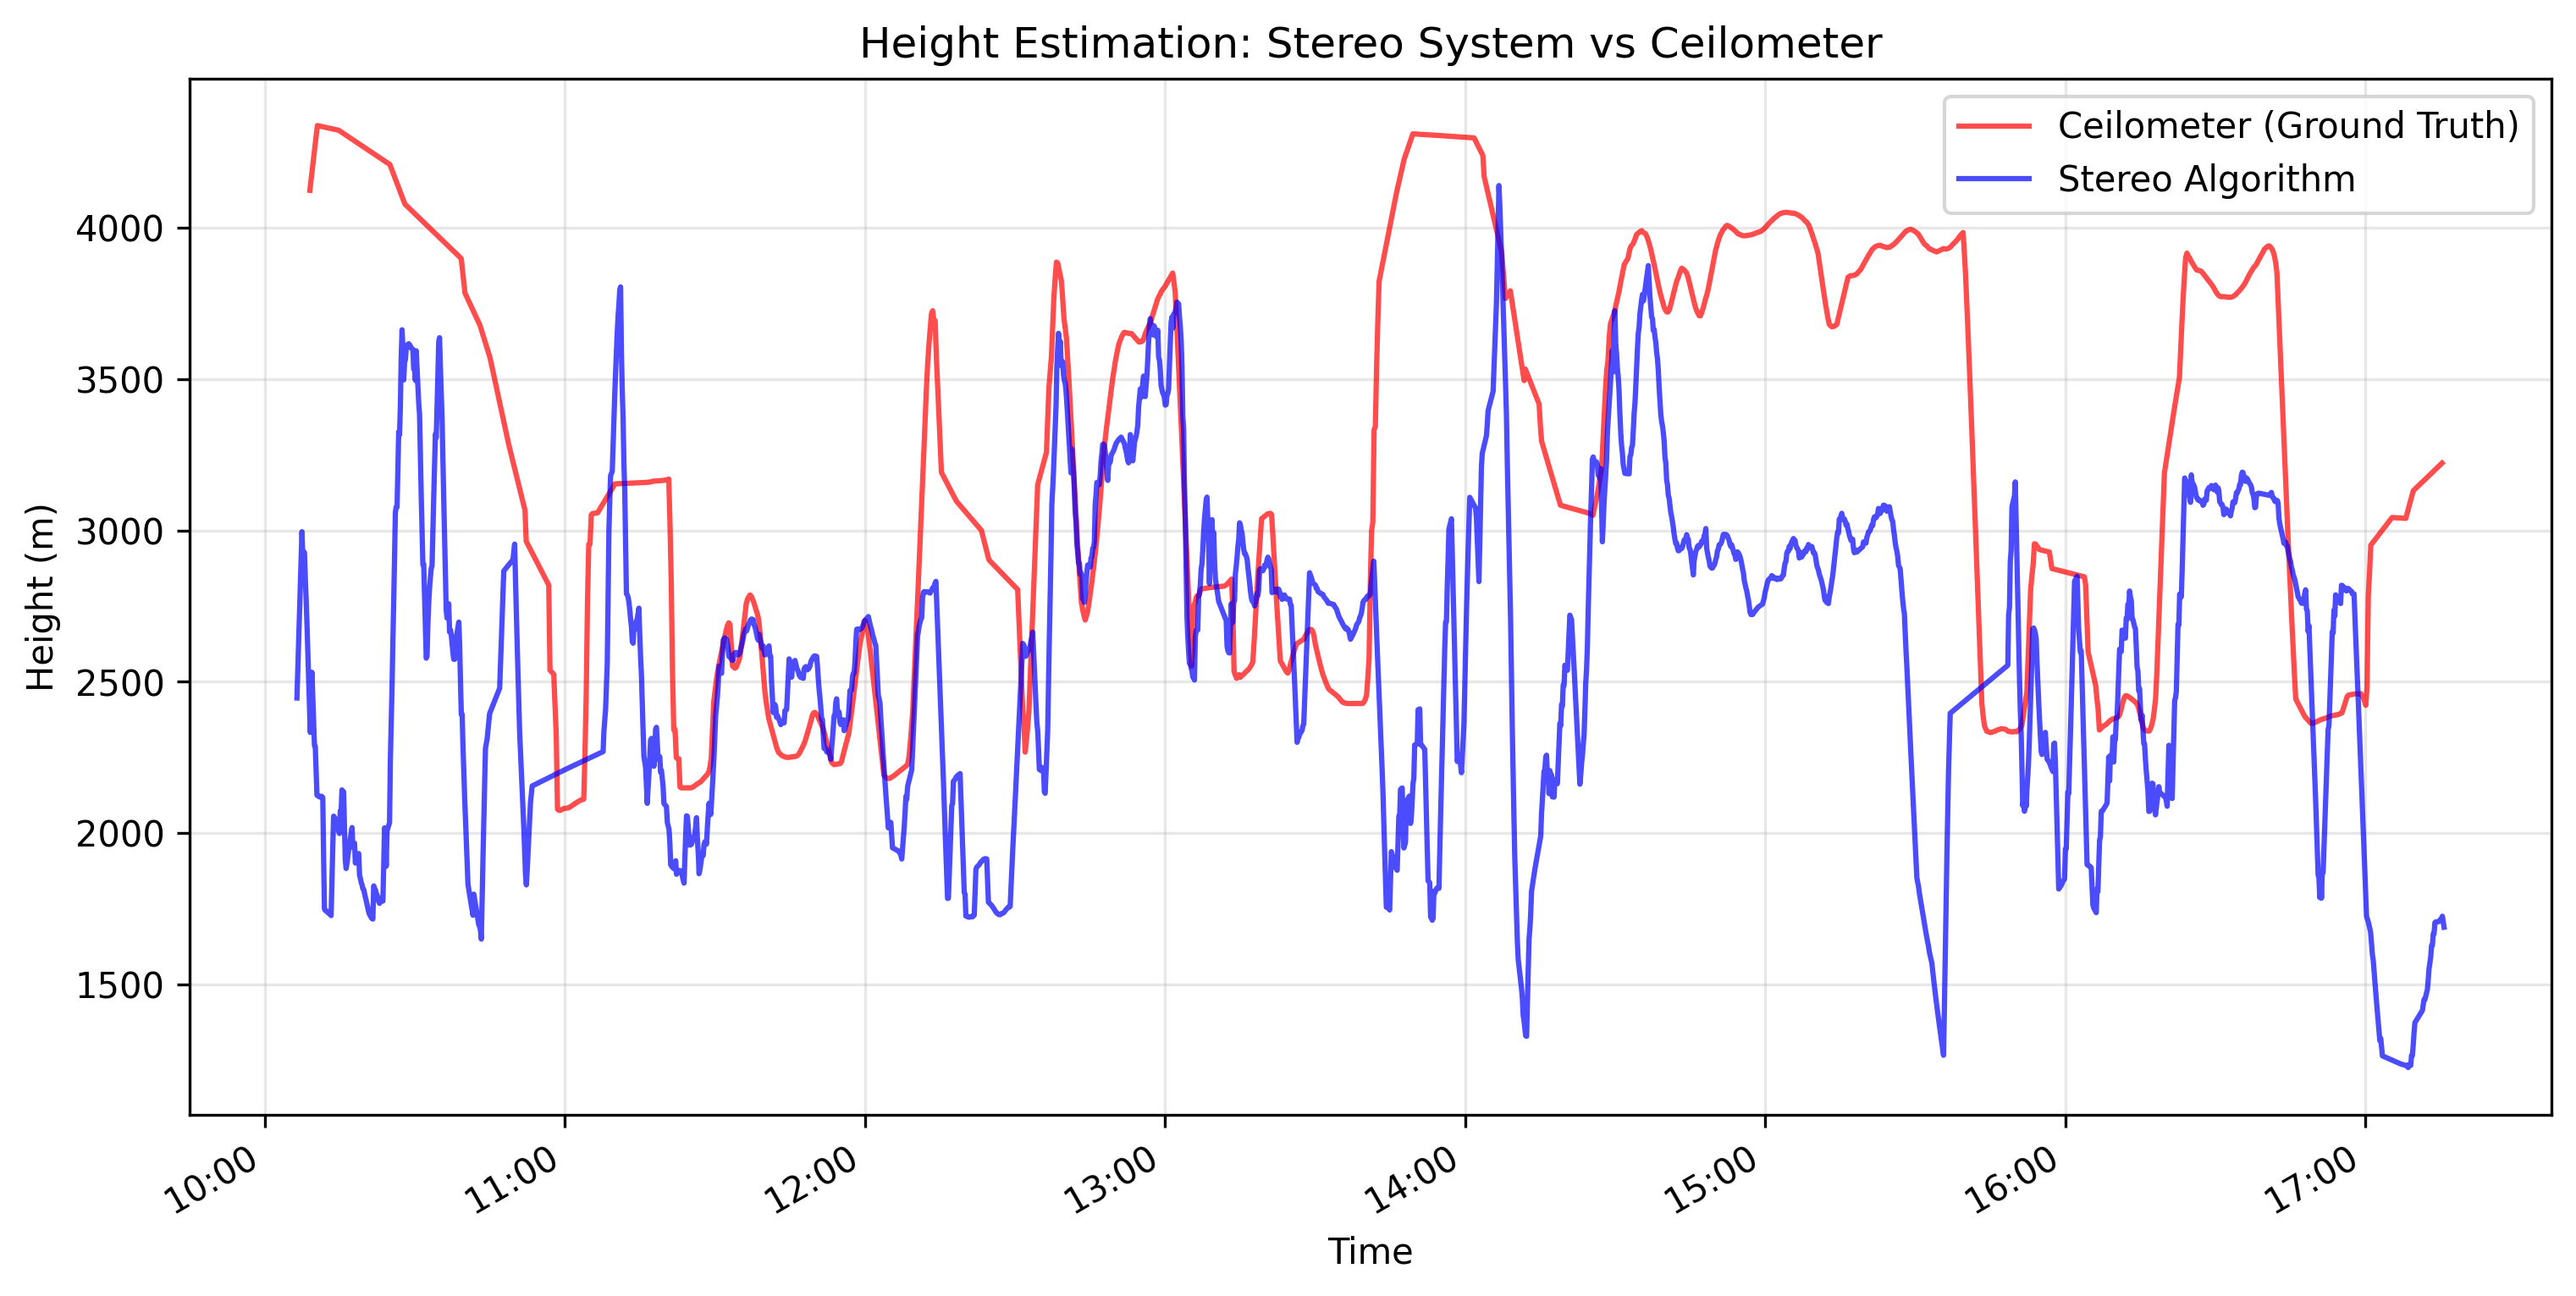
\includegraphics[width=\linewidth]{timeseries_raw}
		\caption{Сравнение временных рядов высоты: данные высотомера (красный) и данные стереосистемы (синий) после сглаживания.}
		\label{fig:timeseries}
	\end{figure}
	
	\subsection{Синхронизация и корреляционный анализ}
	\vspace{3mm}\hspace{5mm}
	
	В ходе первичного сопоставления временных рядов было сделано предположение о расхождении во времени регистрации событий между стереосистемой и высотомером. Для устранения рассинхронизации был применен метод кросс-корреляционного анализа и поиск постоянного временного сдвига для всей последовательности.
	
	Оптимальный временной сдвиг $\tau_{opt}$ определялся как аргумент, максимизирующий коэффициент корреляции Пирсона $r$ между рядами:
	\begin{equation}
		\tau_{opt} = \arg \max_{\tau} \rho(H_{stereo}(t + \tau), H_{ref}(t))
	\end{equation}
	
	
	\begin{figure}[h!]
		\center
		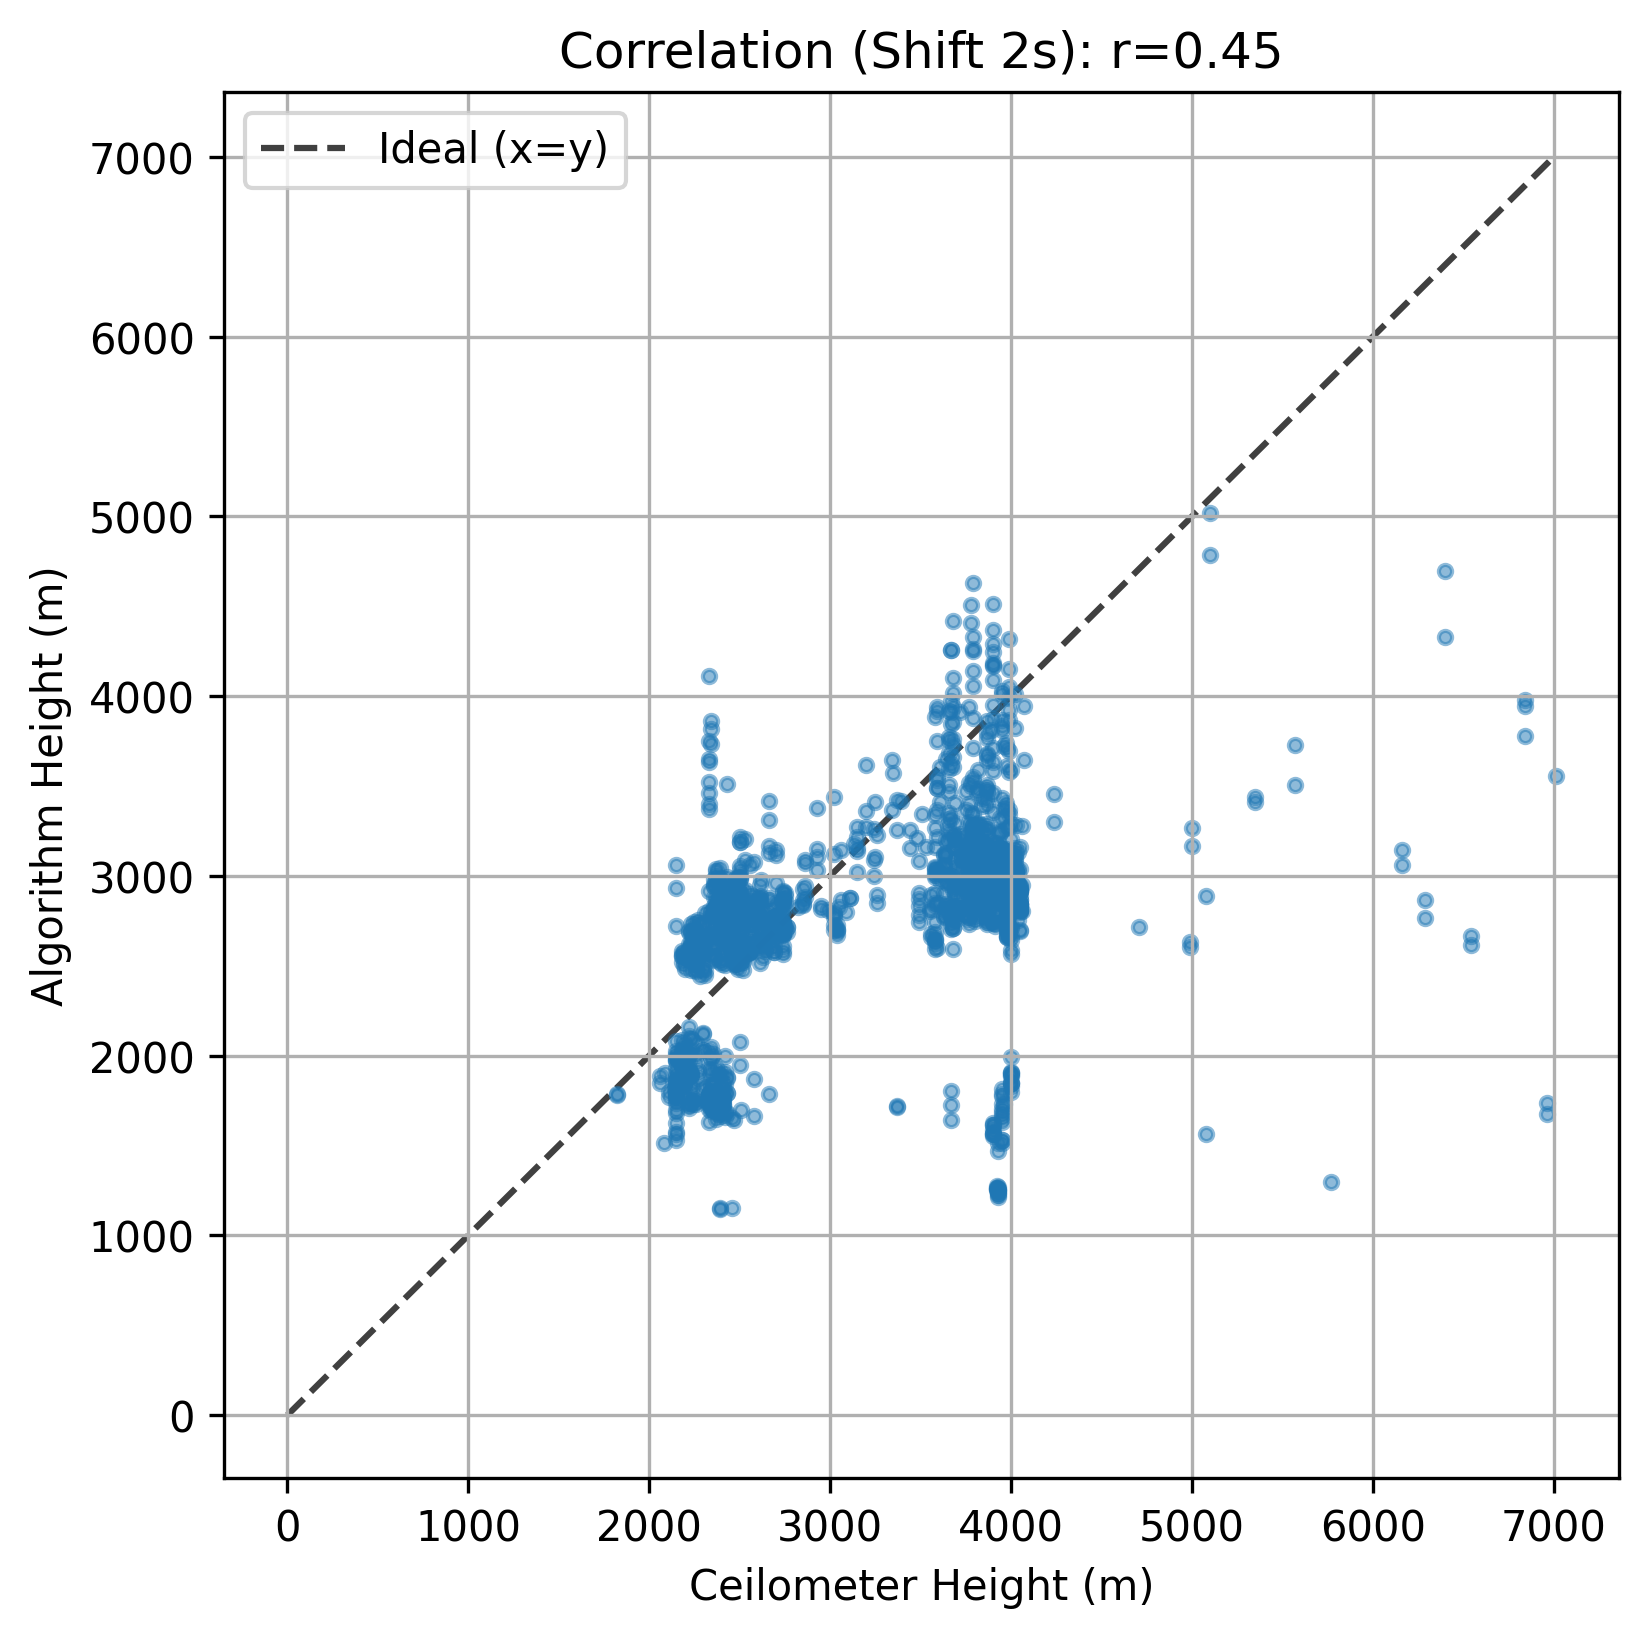
\includegraphics[scale=0.6]{correlation_shifted}
		\caption{Диаграмма рассеяния высот после статической временной синхронизации.}
		\label{fig:correlation}
	\end{figure}
	
	В результате анализа был выявлен временной сдвиг $\tau \approx 2$ секунд. Это говорит о том, что различие во временах регистрации изменений высоты, связанное с фактическим различием расположения стереопары и высотомера, нельзя устранить за счет постоянного временного сдвига. На рис. \ref{fig:correlation} представлена диаграмма рассеяния высот после компенсации этого сдвига. Коэффициент корреляции составил $r \approx 0.45$.
	Геометрически такое расхождение может быть объяснено разным направлением движения облаков: в зависимости от направления, с которого приходят облака, временной сдвиг между регистрацией изменения высоты стереосистемой и высотомером оказывается различным.
	
	\begin{figure}[h!]
		\center
		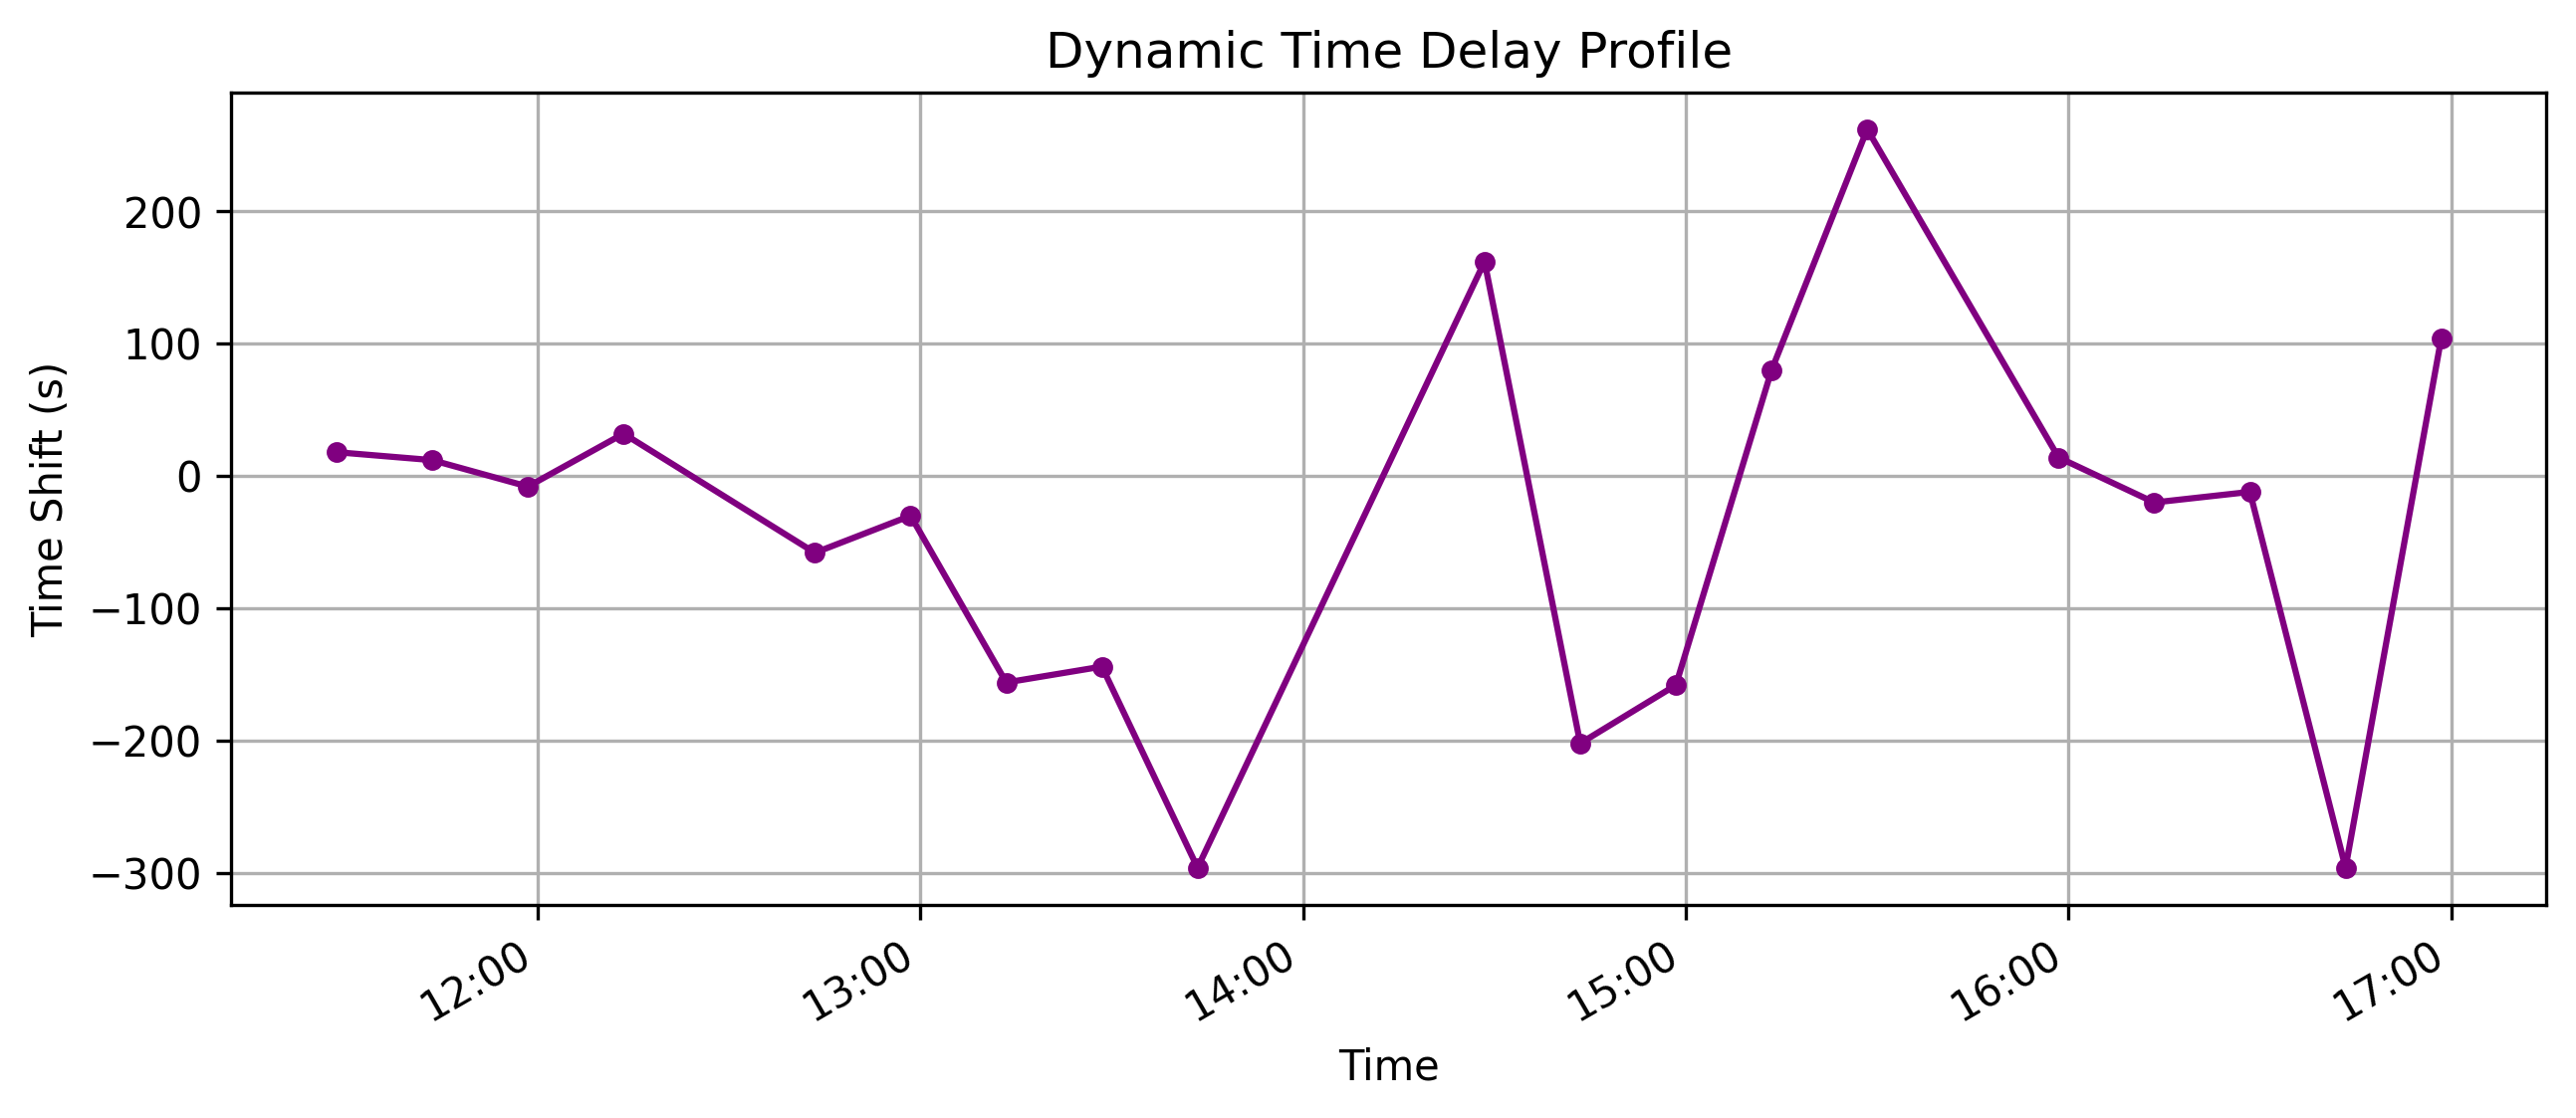
\includegraphics[scale=0.6]{dynamic_shift_profile}
		\caption{Профиль динамического временного смещения.}
		\label{fig:correlation_dynamic_profile}
	\end{figure}
	
	\begin{figure}[h!]
		\center
		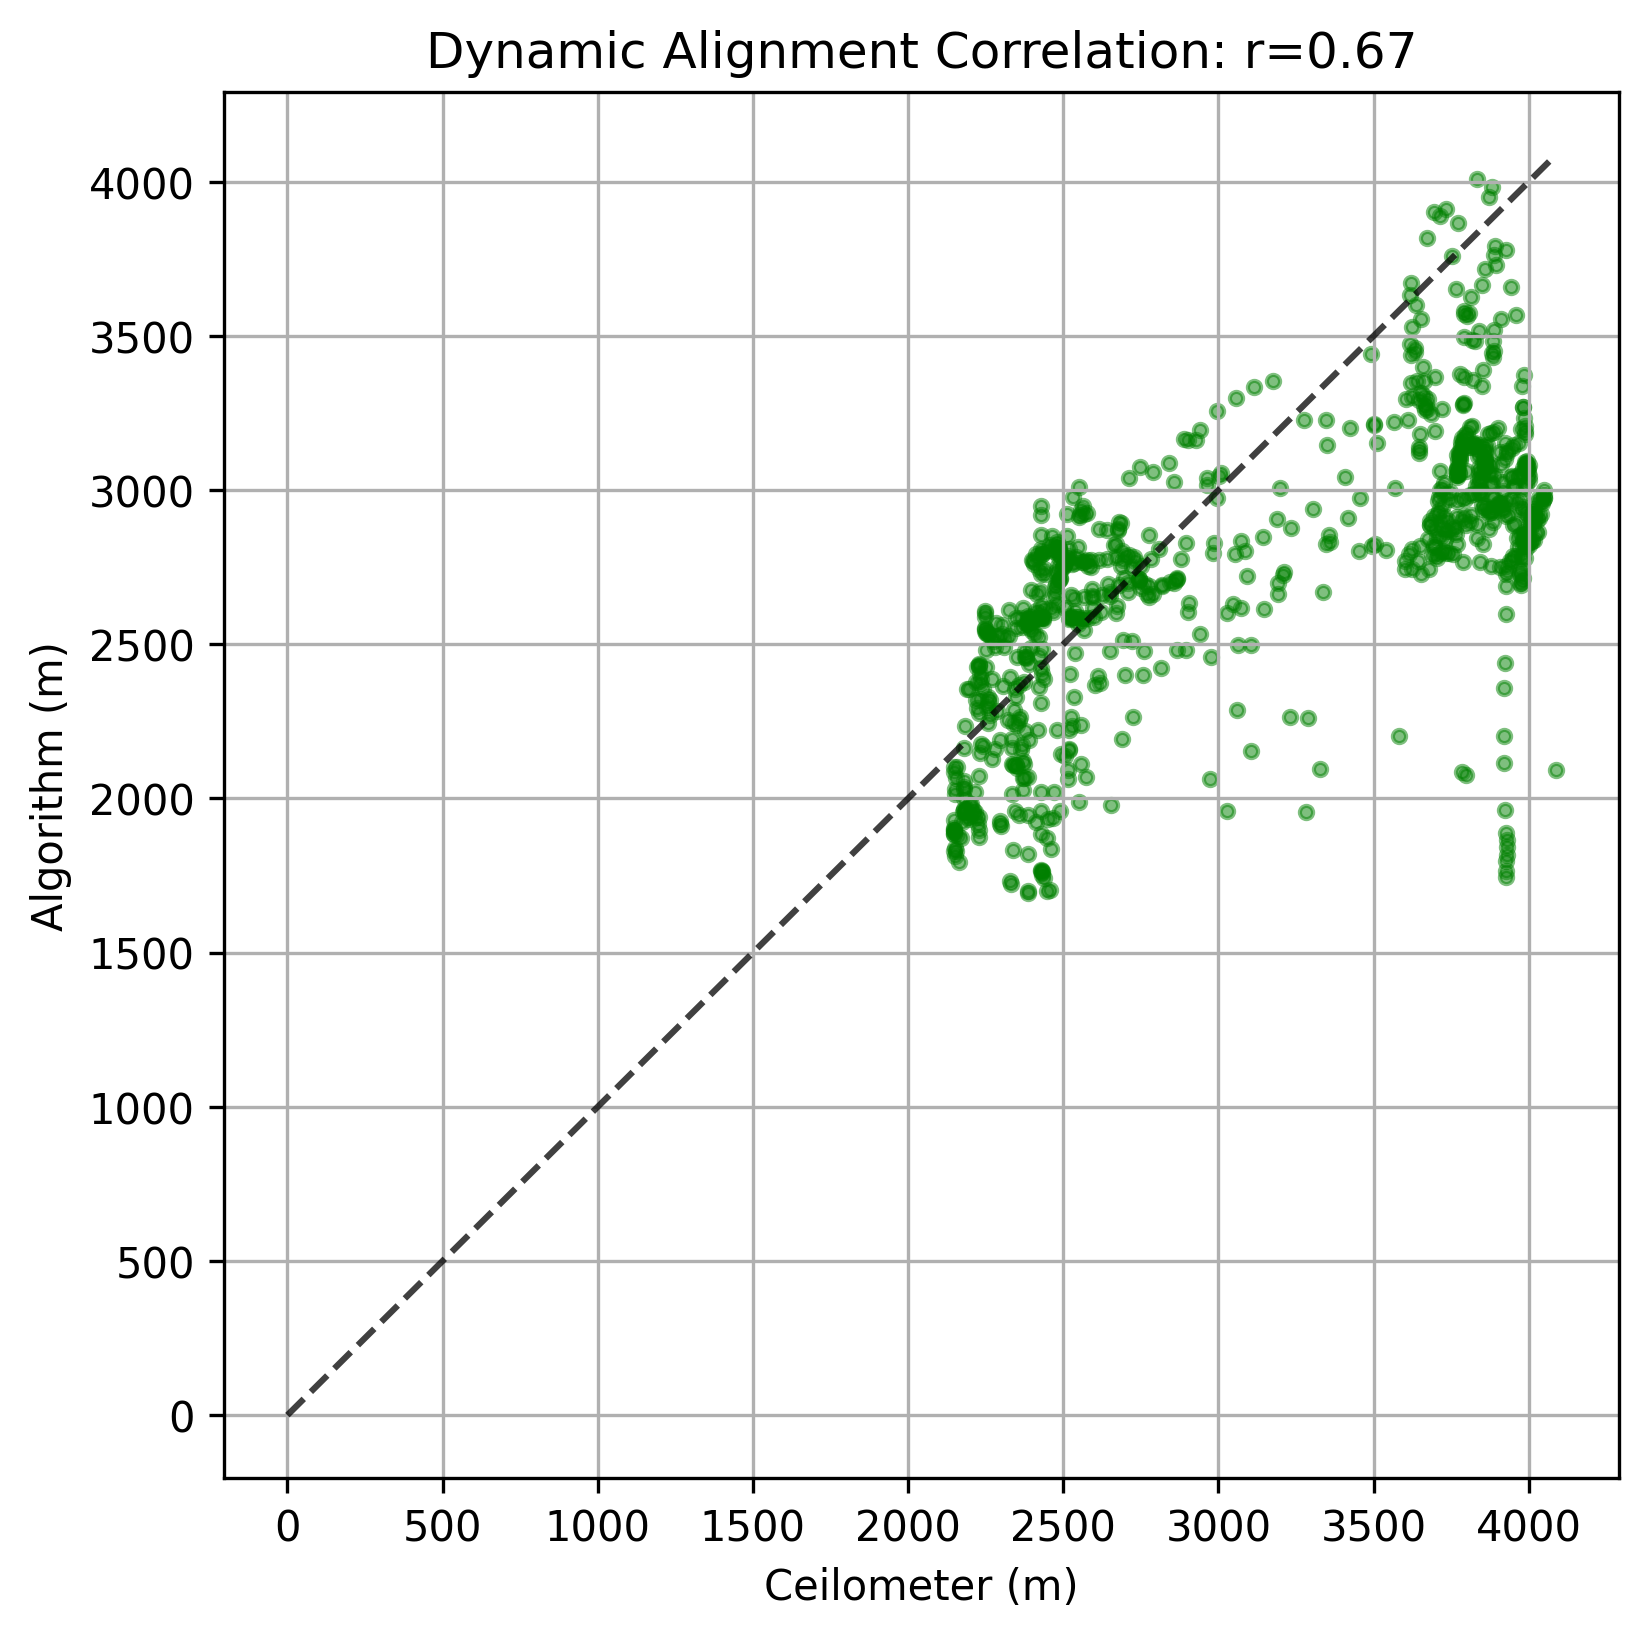
\includegraphics[scale=0.6]{correlation_dynamic}
		\caption{Диаграмма рассеяния высот после динамической временной синхронизации.}
		\label{fig:correlation_dynamic}
	\end{figure}
	
	\begin{figure}[h!]
		\center
		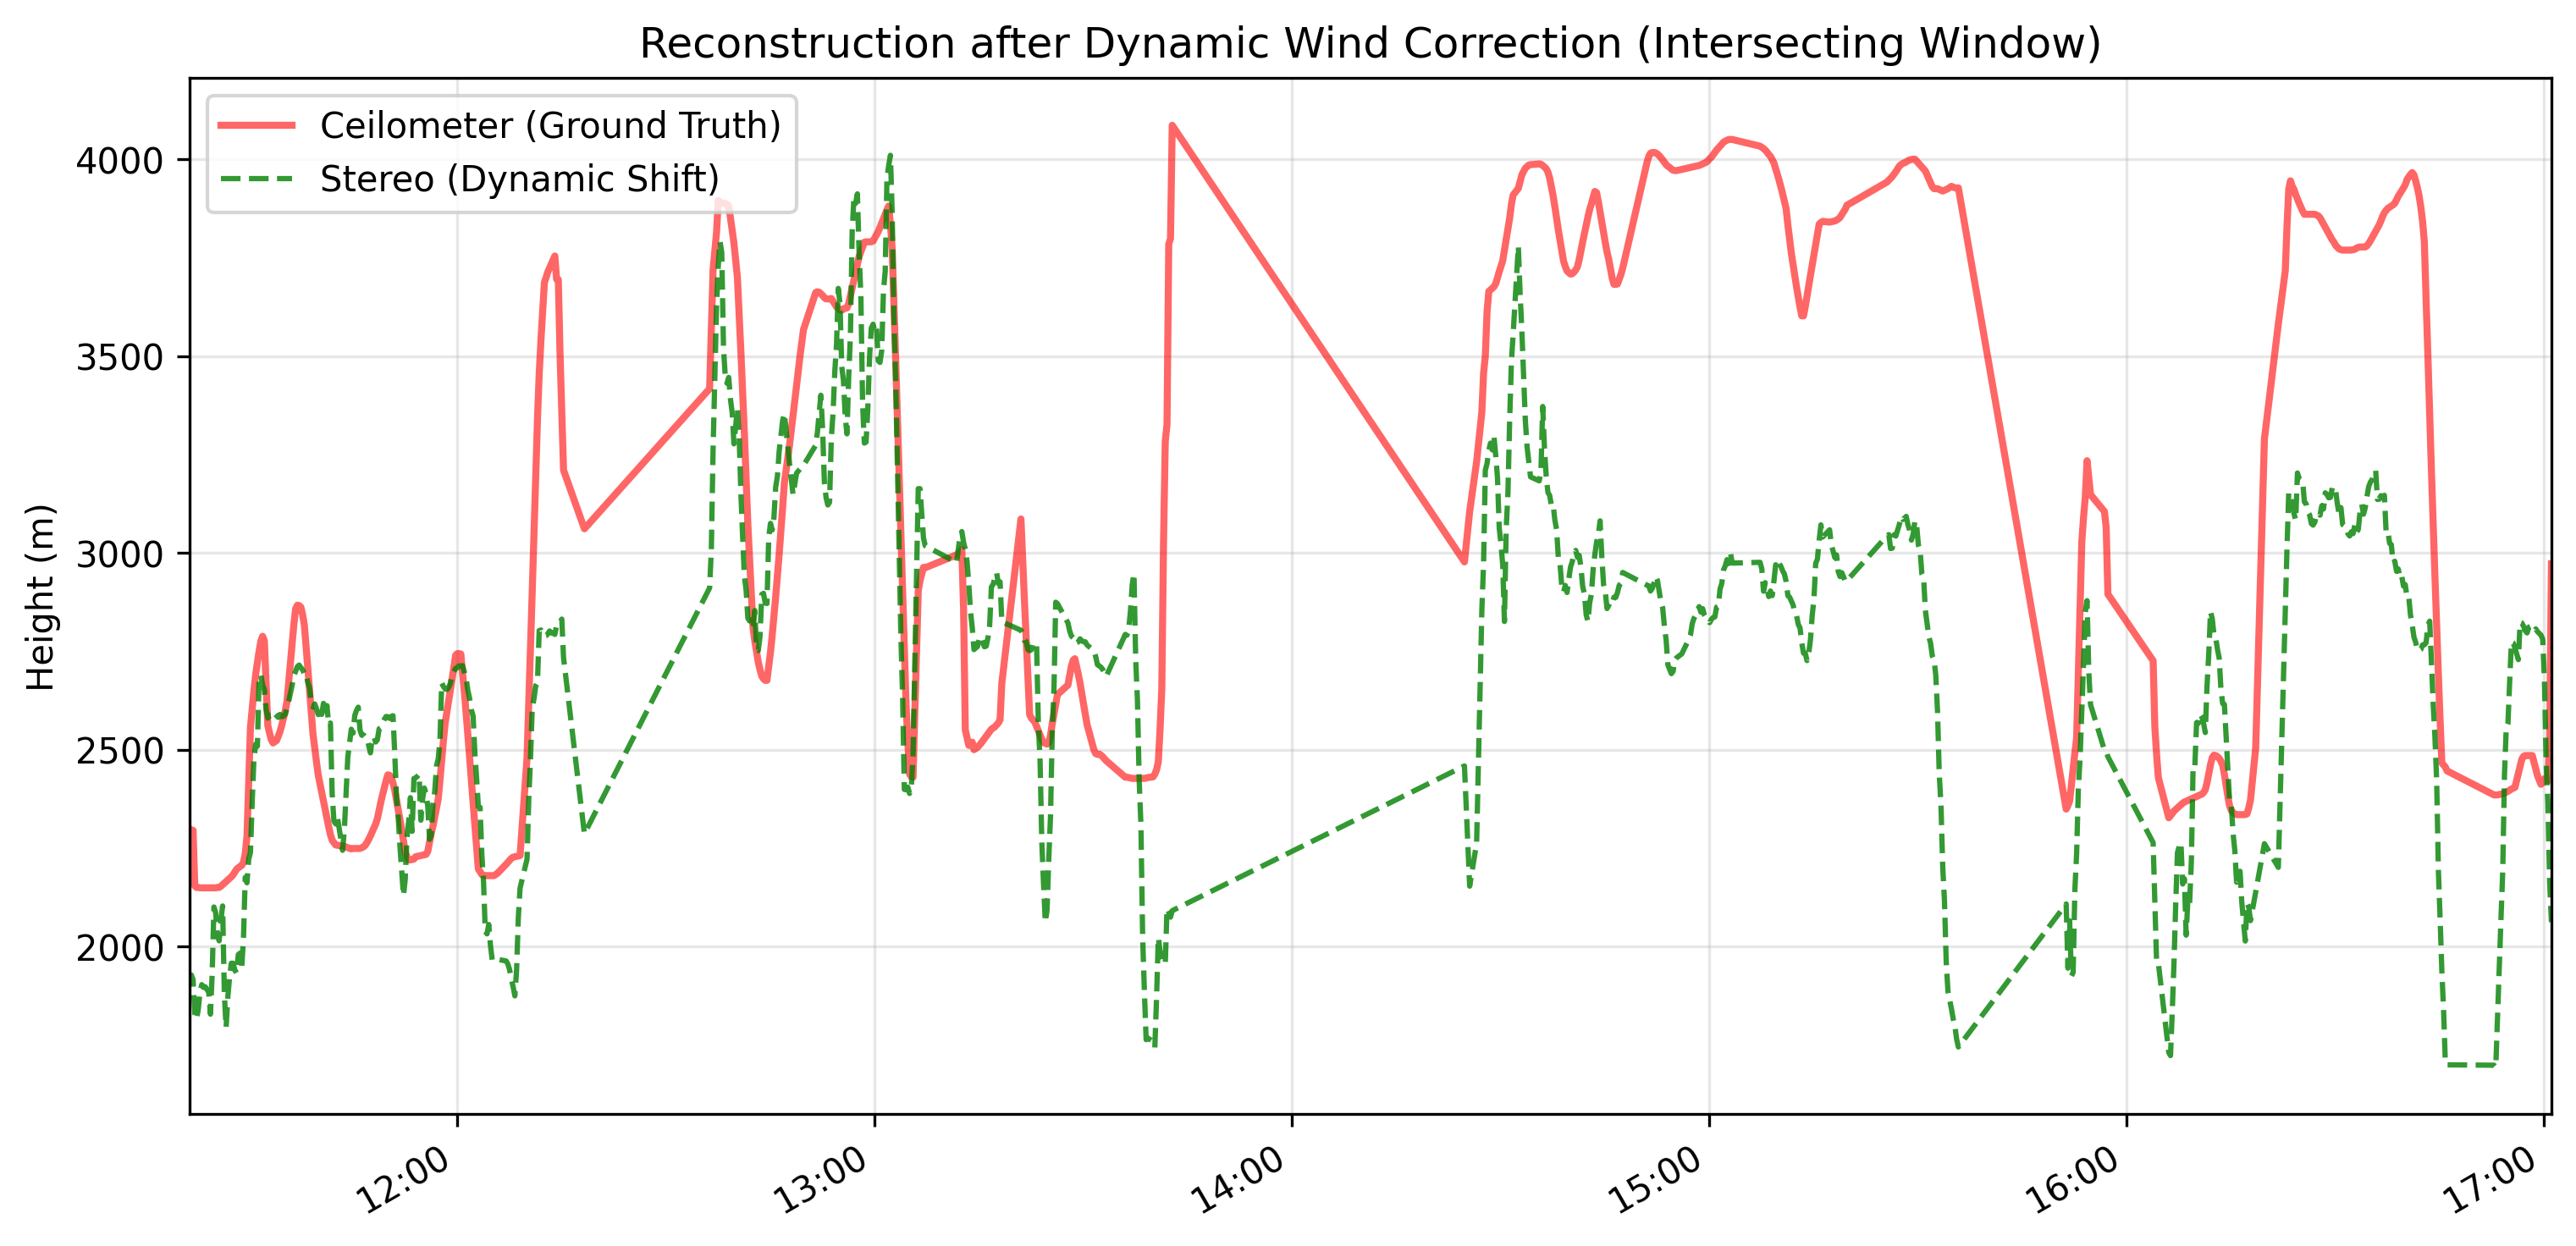
\includegraphics[scale=0.6]{timeseries_dynamic}
		\caption{Сравнение временных рядов высоты: данные высотомера (красный) и данные стереосистемы (зеленый)  после динамической временной синхронизации.}
		\label{fig:timeseries_dynamic}
	\end{figure}
	
	По этой причине временной сдвиг не постоянен. Есть смысл подбирать временной сдвиг для каждого участка данных по отдельности. Выбрано временное окно величиной в 15 минут, в рамках которого искался максимум корелляции по величине временного сдвига (максимум 5 минут). Найден профиль динамического временного сдвига и построен график высот после применения этого динамического профиля. При динамическом временном сдвиге коэффициент корреляции составил $r \approx 0.67$
	
	Сравнение временных рядов после синхронизации (рис. \ref{fig:timeseries_dynamic}) демонстрирует, что стереосистема корректно воспроизводит динамику изменения высоты облачного покрова.
	
	Как видно из графика, алгоритм устойчиво детектирует как резкие изменения высоты, так и плавные тренды. Локальные экстремумы (пики и провалы высоты) на графике алгоритма совпадают с данными высотомера. Наблюдаемое расхождение в абсолютных значениях (смещение графика по вертикали) носит преимущественно систематический характер, однако сохранение общей структуры сигнала подтверждает работоспособность предложенного метода оценки расстояния.
	
	
	\pagebreak
	
	\section{Пространственная фильтрация кластеров}
	\vspace{3mm}\hspace{5mm}
	
	Кластеризация HDBSCAN в пространстве векторов смещений группирует точки по близости смещения, но не учитывает физическую связность соответствующих точек на исходном изображении. Два физически разнесённых участка облачности на одинаковой высоте порождают одинаковое смещение и могут быть объединены в один кластер, хотя реально соответствуют разным облачным полям. Аналогично, ложные соответствия на участках чистого неба (артефакты линз, шум сенсора) могут выживать после HDBSCAN и формировать паразитные кластеры.
	
	Для решения этой проблемы разработан трёхстадийный пространственный фильтр, применяемый к каждому кластеру перед подачей на вход временному трекеру:
	
	\begin{enumerate}
		\item \textbf{Субкластеризация DBSCAN в пространстве изображения.} Для каждого кластера запускается DBSCAN по координатам ключевых точек на первом изображении ($\varepsilon = 30$ px, $\text{min\_samples} = 3$). Сохраняется только наибольший субкластер; точки, отнесённые к шуму (label $=-1$) и миноритарным субкластерам, отбрасываются. Если оставшееся число точек меньше порога, кластер целиком отвергается.
		\item \textbf{Проверка плотности.} Для оставшихся точек строится выпуклая оболочка (ConvexHull) и вычисляется плотность: $\rho = n_\text{pts} / \text{area}$. Если $\rho < 0.002$ точек/пиксель$^2$, кластер отвергается. Рассеянные <<пылевые>> кластеры, где несколько точек покрывают огромную область изображения при близком смещении, не могут соответствовать физическому облаку.
		\item \textbf{Проверка совместной согласованности смещений в пространстве изображения.} Для каждой точки кластера находятся $K = 5$ ближайших соседей в пространстве изображения. Если стандартное отклонение смещения среди соседей превышает $2.0 \cdot \sigma_\text{disp}$ кластера, точка считается неконсистентной. Здесь $\sigma_\text{disp}$ --- стандартное отклонение горизонтальной компоненты смещения $\Delta\xi$ в кластере, характеризующее типичный разброс смещений для данного облачного слоя. Если доля неконсистентных точек превышает 30\%, кластер отвергается. Этот критерий проверяет фундаментальное свойство реальной 3D-поверхности: <<близкие в изображении $\Rightarrow$ близкие по смещению>>.
	\end{enumerate}
	
	Интеграция пространственного фильтра повышает устойчивость временного трекера, устраняя кластеры-артефакты до того, как они смогут породить ложные треки или исказить статистику невязки (innovation) фильтра Калмана --- величины $|z - \hat{x}^-|$, характеризующей отклонение текущего измерения от предсказанного значения и используемой для адаптивной настройки доверия к измерениям (см. раздел~\ref{sec:kalman}).
	
	\pagebreak
	
	\section{Временная фильтрация на основе фильтра Калмана}
	\vspace{3mm}\hspace{5mm}
	
\subsection{Постановка задачи}
\vspace{3mm}\hspace{5mm}

\textbf{Неформальная постановка.} Дана последовательность независимых точечных оценок высоты нижней границы облачности, полученных по каждой стереопаре. Оценки зашумлены и содержат выбросы; соседние по времени оценки могут физически нереалистично различаться (до 500 м за 10 с). Требуется получить сглаженную временную траекторию высоты, устраняющую выбросы и согласованную с физическими ограничениями на скорость изменения высоты облачного слоя.

\textbf{Формальная постановка.} Пусть $\{z_t\}_{t=1}^T$ — последовательность измерений высоты облачности по стереопаре в дискретные моменты времени $t$. Известна физическая модель эволюции высоты — равномерное движение: $h_{t+1} = h_t + \dot{h}_t \Delta t$, $\dot{h}_{t+1} = \dot{h}_t$. Погрешность измерений включает как шум с неизвестной дисперсией, так и аномальные выбросы. Требуется восстановить скрытое состояние $\mathbf{x}_t = [h_t, \dot{h}_t]^\top$, минимизируя среднеквадратичную ошибку оценки при неизвестной статистике шума измерений и наличии выбросов в $\{z_t\}$.


\subsection{Мотивация}

В исходной постановке каждая стереопара анализируется независимо: LOFTR извлекает соответствия, HDBSCAN кластеризует по смещениям, и высота доминирующего кластера становится оценкой CBH для данного кадра. Никакая временная информация не используется — оценка в момент $t$ не имеет <<памяти>> об оценках в $t-1, t-2, \dots$ Следствием являются:
	\begin{itemize}
		\item физически нереалистичные скачки высоты между соседними кадрами (до 500 м за 10 с, что эквивалентно вертикальной скорости $>50$ м/с);
		\item фрагментация одного облачного слоя на несколько HDBSCAN-кластеров в последовательных кадрах;
		\item низкая автокорреляция временного ряда ($r_\text{auto} \approx 0.11$ на 5-часовом интервале; автокорреляция — корреляция высоты с самой собой при сдвиге в один кадр, характеризующая гладкость ряда), что затрудняет сопоставление с высотомером.
	\end{itemize}
	
	\subsection{Одномерный инновационно-адаптивный фильтр Калмана}
	\label{sec:kalman}
	
	Разработан фильтр Калмана, моделирующий эволюцию высоты облачности как процесс равномерного движения:
	
	\begin{equation}
		h(t + \Delta t) = h(t) + \dot{h}(t) \cdot \Delta t, \quad \dot{h}(t + \Delta t) = \dot{h}(t)
	\end{equation}
	
	Вектор состояния: $\mathbf{x} = [h, \dot{h}]^\top$. Матрица перехода:
	
	\begin{equation}
		\mathbf{F} = \begin{pmatrix} 1 & \Delta t \\ 0 & 1 \end{pmatrix}
	\end{equation}
	
	Процессный шум $\mathbf{Q}$ параметризован через ускорение $\sigma_h$:
	
	\begin{equation}
		\mathbf{Q} = \sigma_h^2 \begin{pmatrix} \Delta t^4/4 & \Delta t^3/2 \\ \Delta t^3/2 & \Delta t^2 \end{pmatrix}, \quad \sigma_h = 5.0\ \text{м/с}^2
	\end{equation}
	
	\textbf{Адаптивная матрица измерений.} Вместо фиксированной ковариации измерений $R$ (величина, определяющая, насколько фильтр доверяет текущему измерению $z$ относительно предсказания $\hat{x}^-$) используется инновационно-адаптивная схема: шум измерений пропорционален квадрату отклонения текущего измерения от предсказания:
	
	\begin{equation}
		R = \text{clip}(R_\text{scale} \cdot \max(|z - \hat{x}^-|, 10)^2 \cdot 0.01,\ 100,\ 10^6)
	\end{equation}
	
	где $z$ --- измерение высоты от стереосистемы, $\hat{x}^-$ --- предсказанное значение высоты, $R_\text{scale} = 50$ --- масштабирующий коэффициент. Функция $\text{clip}(x, a, b)$ ограничивает значение $x$ снизу и сверху: $\text{clip}(x, a, b) = \max(a, \min(x, b))$ --- если $x$ выходит за пределы интервала $[a, b]$, то оно заменяется на ближайшую границу. В формуле (12) интервал $[100, 10^6]$ задаёт допустимый диапазон для $R$, исключая вырожденные случаи $R \to 0$ (приводящие к сингулярности) и $R \to \infty$ (приводящие к игнорированию измерений). При малой инновации $|z - \hat{x}^-|$ (измерение близко к предсказанию) $R$ мало — фильтр доверяет измерению. При большой инновации (вероятный выброс) $R$ велико — фильтр опирается на предсказание. Это позволяет автоматически подавлять выбросы без жёсткого порога отсечения.
	
	\textbf{Неопределённость измерений на основе SEM.} Стереопогрешность высоты вычисляется через стандартную ошибку среднего (SEM --- Standard Error of the Mean) смещений в кластере: $\sigma_h = f(\sigma_{\text{disp}} / \sqrt{n_\text{pts}})$, где $\sigma_{\text{disp}}$ --- стандартное отклонение смещений в кластере, $n_\text{pts}$ --- число точек, а $f$ --- функция пересчёта смещения в высоту (формула 3). Для типичного кластера из 566 точек $\sigma_h^{\text{SEM}} \approx 5$ м против $\sigma_h^{\text{std}} \approx 124$ м при использовании обычного стандартного отклонения — 25-кратное снижение неопределённости, критичное для корректного баланса коэффициента Калмана.
	
	\subsection{Слияние кластеров и стратегия выбора}
	
	Перед подачей на вход фильтру кластеры, различающиеся по высоте менее чем на 300 м, сливаются — это противодействует фрагментации одного облачного слоя на несколько HDBSCAN-кластеров. Доступны три стратегии выбора целевого кластера: \texttt{largest} (наибольший по числу точек), \texttt{lowest} (наинизший для метеорологической нижней границы) и \texttt{lowest\_reliable} (наинизший с числом точек выше порога).
	
	\subsection{Результаты временной фильтрации}
	
	Фильтр протестирован на данных 23 мая 2025 года (12:00--17:00). Основные результаты:

	\vspace{2mm}
	\begin{table}[h!]
		\centering
		\begin{tabular}{||l c c c||} 
			\hline
			Метрика & Исходные данные & Фильтрованные & Улучшение \\
			\hline\hline
			Средний перепад высоты $|\Delta h|$ (10-с кадры) & 515 м & 120 м & \textbf{в 4.3 раза} \\
			Автокорреляция (5 ч) & 0.11 & 0.90 & \textbf{в 8.0 раз} \\
			Средняя $r$ в 30-мин окнах & 0.55 & 0.61 & +11\% \\
			Доля окон с $r > 0.5$ & 61\% (11/18) & 72\% (13/18) & --- \\
			Максимальная $r$ в окне & 0.88 & 0.94 & --- \\
			\hline
		\end{tabular}
		\caption{Сравнение метрик до и после применения фильтра Калмана}
		\label{table:2}
	\end{table}
	
	Фильтр уменьшает разброс высот между кадрами в 4.3 раза, повышает автокорреляцию временного ряда в 8 раз и даёт прирост средней корреляции с высотомером на 11\%. В 72\% 30-минутных окон корреляция превышает 0.5, достигая 0.94 в наиболее благоприятных атмосферных условиях.
	
	\begin{figure}[h!]
		\center
		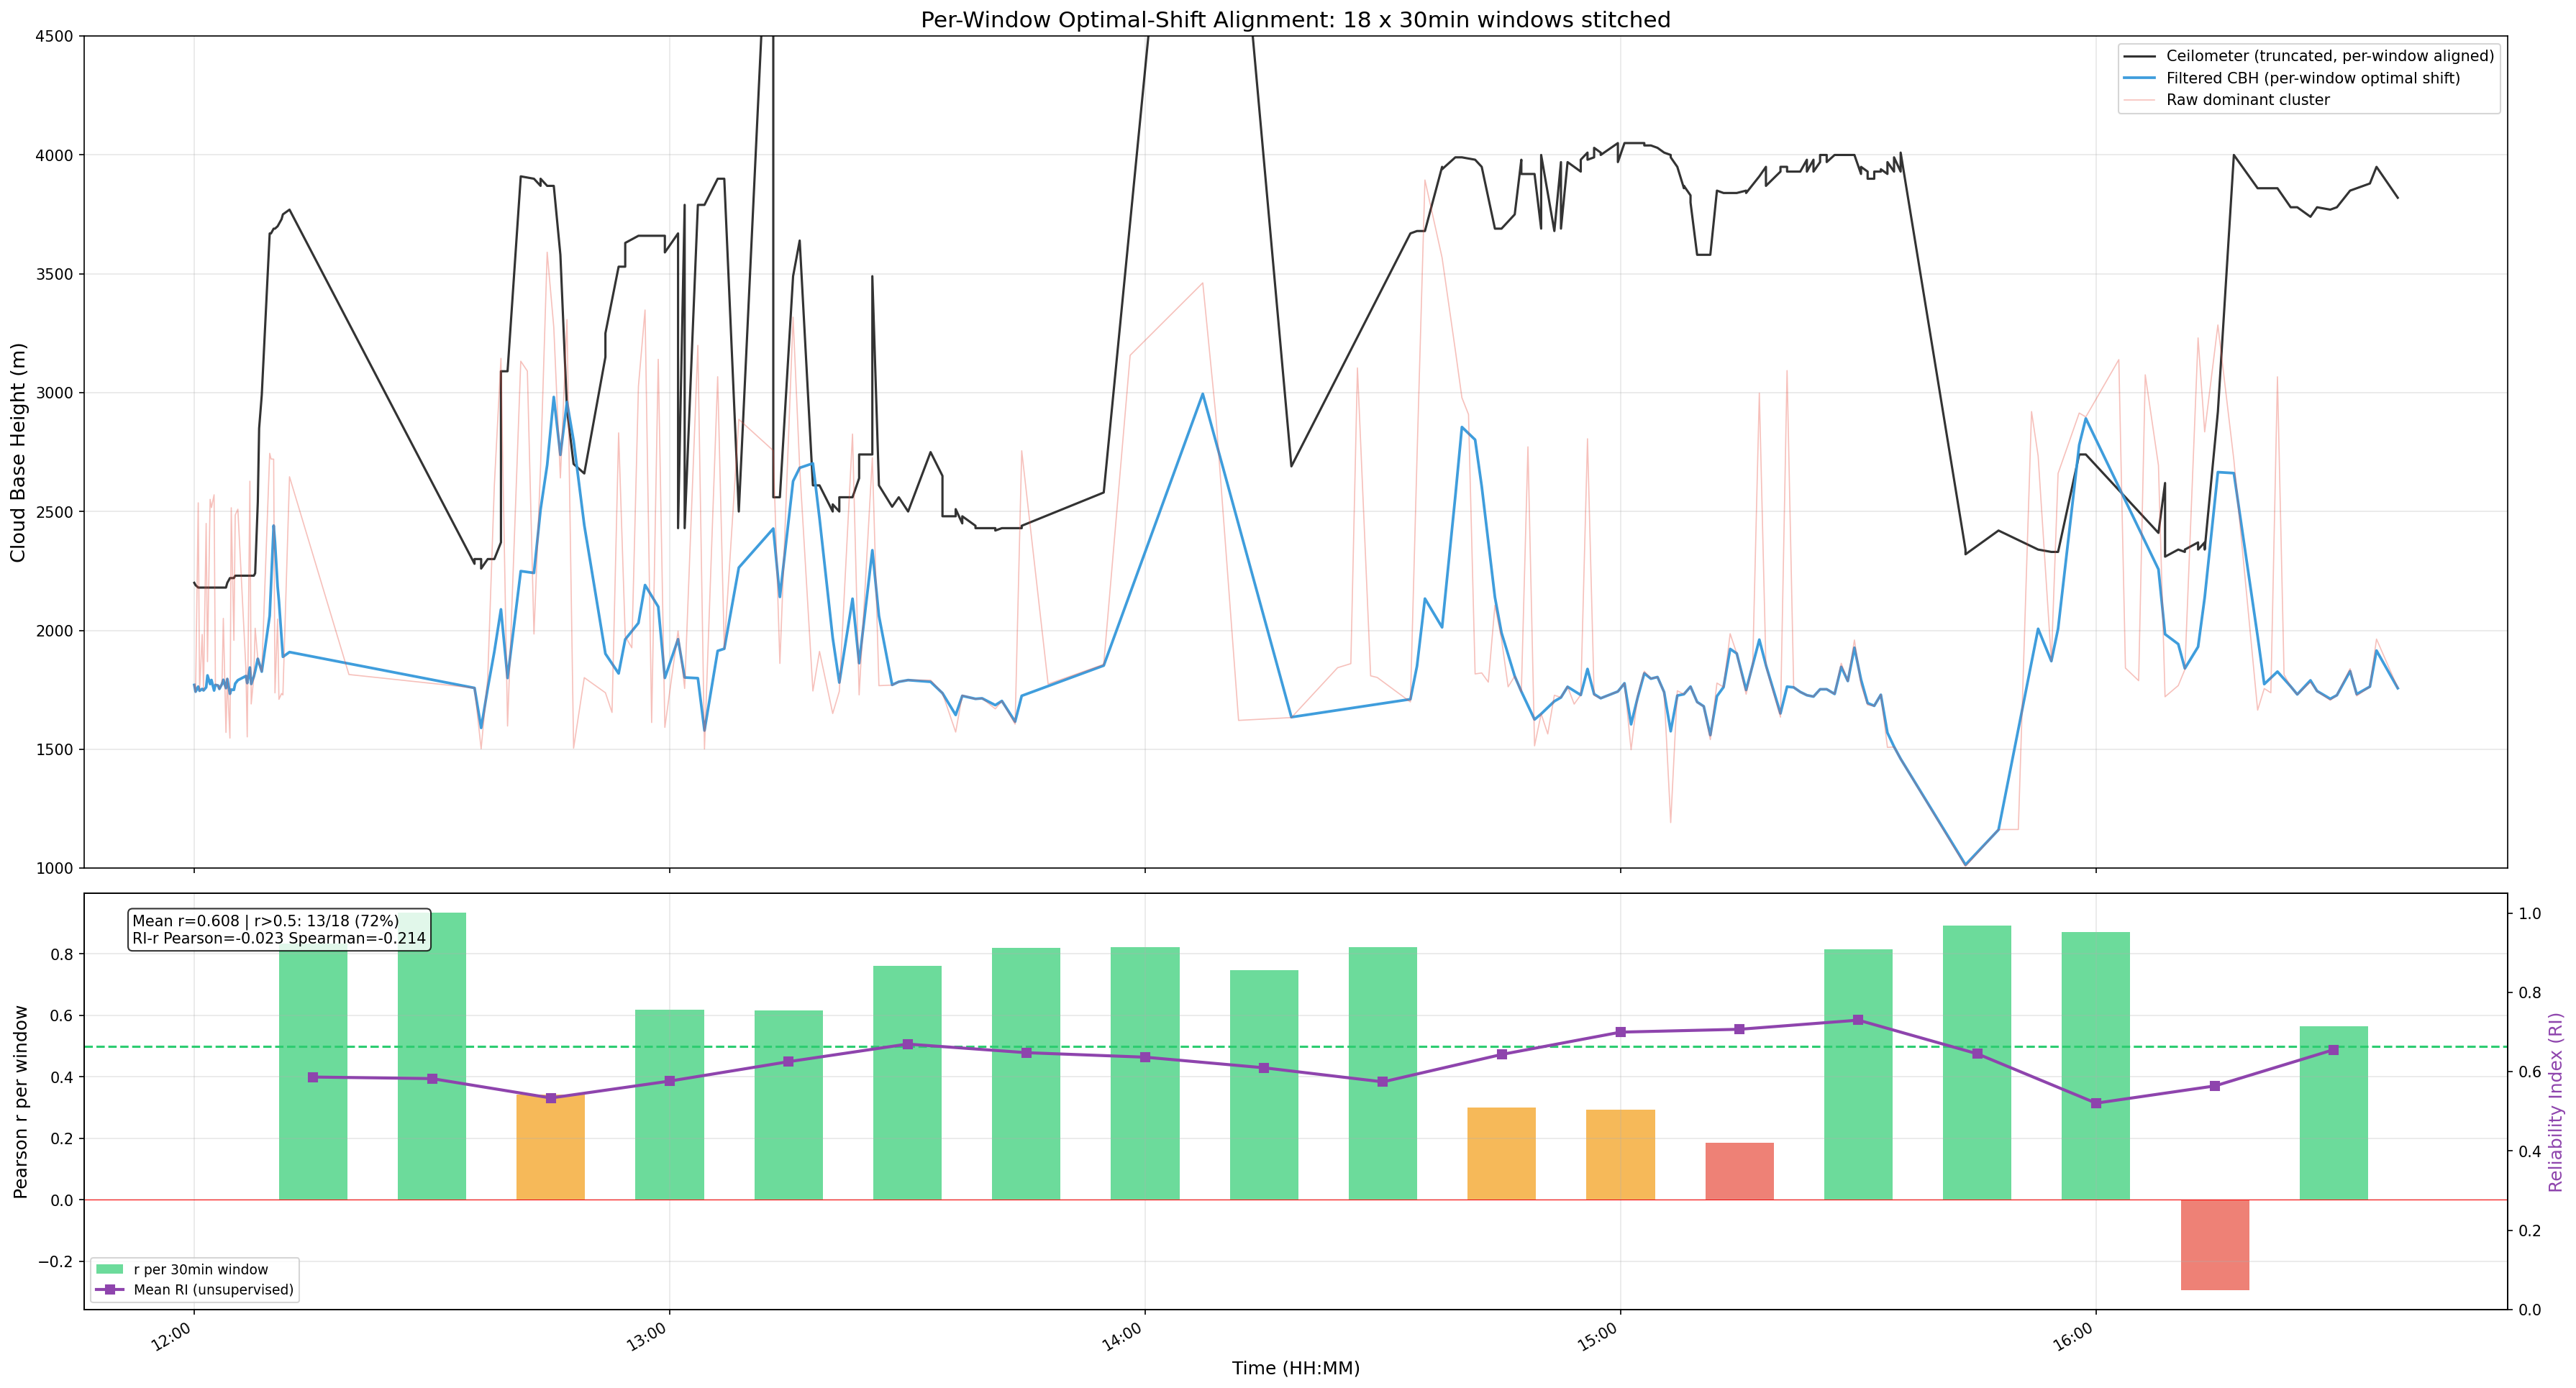
\includegraphics[width=0.95\linewidth]{01_stitched_windows}
		\caption{Сшитый временной ряд высоты нижней границы облачности по 30-минутным окнам с индивидуальной временной синхронизацией. \textbf{Верхняя панель:} временные ряды высоты — данные высотомера (красный), данные стереосистемы (зелёный) и отфильтрованная стереооценка (синий). \textbf{Нижняя панель:} коэффициент корреляции Пирсона $r$ между стереосистемой и высотомером (оранжевый) для каждого 30-минутного окна, характеризующий согласованность алгоритмической оценки с эталонными измерениями.}
		\label{fig:stitched}
	\end{figure}
	
	

\section{О систематическом смещении показаний высотомера}
	\vspace{3mm}\hspace{5mm}
	
	В эксперименте в качестве эталонного прибора использовался лазерный облакомер (датчик высоты облаков) \textbf{ДОЛ-2} [12]. Прибор основан на измерении обратно рассеянного зондирующего импульса полупроводникового лазера при прохождении им исследуемого участка трассы. Технические характеристики ДОЛ-2: диапазон измерений 10--3000 м; разрешающая способность 7.5 м; пределы допускаемой абсолютной погрешности $\pm 10$ м в диапазоне 10--100 м и $\pm(5.0 + 0.05 H)$ м в диапазоне 100--3000 м; частота обновления данных --- 15 с [12].
	
	При интерпретации расхождений между стереосистемой и высотомером необходимо учитывать физику работы самого высотомера. Высотомер измеряет не геометрическую границу облака, а \textbf{оптический профиль обратного рассеяния} атмосферы.
	
	Лазерный импульс высотомера, достигая нижней кромки облака, не отражается мгновенно — облачные основания часто диффузны, с плавным нарастанием концентрации водяных капель. Для того чтобы алгоритм высотомера зарегистрировал «нижнюю границу», сигнал обратного рассеяния должен уверенно отразиться от облака, а это не всегда происходит на самой нижней границе — сигнал достигает порога детекции лишь на некоторой глубине внутри облачного слоя.
	
	Следствием является \textbf{систематическое завышение} высоты высотомером относительно истинной геометрической границы облака:
	\begin{itemize}
		\item Высотомер всегда даёт значения \textbf{выше или равные} истинной нижней границе облака;
		\item В зависимости от типа облачности и концентрации влаги завышение составляет от единиц до сотен метров;
		\item Средняя величина ошибки между высотомером и стереосистемой составляет от 0 до $\sim$2000 м в зависимости от временного окна и типа наблюдаемой облачности.
	\end{itemize}
	
	Этот эффект объясняет часть систематического вертикального смещения между данными стереосистемы и высотомера и должен учитываться при интерпретации абсолютных значений высоты.
	
	\pagebreak
	
\section{Многотрековое расширение}
\vspace{3mm}\hspace{5mm}

\textbf{Неформальная постановка.} В условиях многослойной облачности на одном кадре могут присутствовать несколько кластеров, соответствующих разным облачным слоям на разных высотах. Требуется одновременно отслеживать эволюцию каждого слоя во времени: сопоставлять кластеры из последовательных кадров (задача ассоциации данных), фильтровать траекторию каждого слоя и определять моменты появления и исчезновения слоёв.

\textbf{Формальная постановка.} Пусть в каждый момент времени $t$ стереосистема порождает множество измерений $\mathcal{Z}_t = \{\mathbf{z}_t^i\}_{i=1}^{N_t}$, где каждое измерение $\mathbf{z}_t^i = [h, u, v, s]^\top$ содержит высоту $h$, координаты центроида $(u, v)$ в плоскости изображения и размер $s$ кластера. Известна модель процесса — постоянная скорость со случайным блужданием ускорения для вектора состояния $\mathbf{x} = [h, \dot{h}, u, v, \dot{u}, \dot{v}, s]^\top$. Требуется: (1) ассоциировать каждое измерение $\mathbf{z}_t^i$ с одним из существующих треков либо инициировать новый трек; (2) выполнить фильтрацию Калмана для каждого трека; (3) определить моменты инициализации и завершения треков по критерию M-of-N.

Для сценариев с устойчивой многослойной облачностью разработан полный многотрековый фильтр Калмана с 7-мерным вектором состояния:
	
	\begin{equation}
		\mathbf{x}(t) = [h, \dot{h}, u, v, \dot{u}, \dot{v}, s]^\top
	\end{equation}
	
	где $h$ — высота, $\dot{h}$ — скорость изменения высоты, $u, v$ — координаты центроида кластера в изображении, $\dot{u}, \dot{v}$ — скорости дрейфа в изображении, $s$ — размер кластера (число точек).
	
	\textbf{Модель процесса} — постоянная скорость со случайным блужданием ускорения. Матрица перехода $\mathbf{F}$ размером $7 \times 7$ блочно-диагональна с блоками $[[1, \Delta t], [0, 1]]$ для каждой пары (позиция, скорость). Процессный шум $\mathbf{Q}$ выведен из физических ограничений: $\sigma_{\ddot{h}} = 0.5$ м/с$^2$ (вертикальное ускорение), $\sigma_{\ddot{u}} = \sigma_{\ddot{v}} = 2.0$ пикс/с$^2$ (турбулентные порывы).
	
	\textbf{Модель измерений:} $\mathbf{z}^i = [h_\text{meas}, u_\text{meas}, v_\text{meas}, s_\text{meas}]^\top$ с адаптивной матрицей ковариации $\mathbf{R} = \text{diag}(\sigma_h^2, \sigma_u^2, \sigma_v^2, \sigma_s^2)$, где $\sigma_h^2$ вычисляется через распространение ошибки стереоформулы.
	
	\textbf{Ассоциация данных} между треками и новыми измерениями выполняется венгерским алгоритмом над матрицей стоимостей, построенной на квадрате расстояния Махаланобиса [8,9]:
	
	\begin{equation}
		d^2 = (\mathbf{z} - \mathbf{H}\hat{\mathbf{x}}^-)^\top \mathbf{S}^{-1} (\mathbf{z} - \mathbf{H}\hat{\mathbf{x}}^-), \quad \mathbf{S} = \mathbf{H}\mathbf{P}^-\mathbf{H}^\top + \mathbf{R}
	\end{equation}
	
	с гейтированием по критерию $\chi^2_4(0.99) \approx 13.28$ и проверками физической правдоподобности: $|\Delta h|/\Delta t \le 10$ м/с, скорость в изображении $\le 100$ пикс/с, отношение размеров кластеров в диапазоне $[0.2, 5.0]$.
	
	\textbf{Жизненный цикл треков} реализует M-of-N инициализацию: новый трек находится в состоянии PROBATION и переходит в CONFIRMED после $M = 2$ ассоциаций в первых $N = 3$ кадрах. Трек переходит в DEAD после $K = 5$ последовательных пропусков. 	Для оптимального сглаживания реализован офлайн RTS-смузер (Rauch-Tung-Striebel) [10] — обратный проход, вычисляющий оптимальную оценку состояния с учётом всех будущих измерений.
	
	В эксплуатационном режиме используется упрощённый одномерный фильтр Калмана (секция \ref{sec:kalman}): нестабильность HDBSCAN-меток между кадрами делает венгерскую ассоциацию ненадёжной для данных с высоким уровнем шума. Многотрековый режим реализован и доступен для сценариев с устойчивой стратификацией облачности.
	
	\pagebreak
	
	\section{Обсуждение результатов}
	\vspace{3mm}\hspace{5mm}
	
	Разработанный комплекс методов — пространственная фильтрация, временной фильтр Калмана и многотрековое расширение — формирует полный конвейер обработки данных стереосистемы для оценки высоты нижней границы облачности. Ключевые выводы:
	
	\begin{enumerate}
		\item \textbf{Временная фильтрация Калмана} является наиболее эффективным улучшением: снижение разброса высот между кадрами в 4.3 раза и повышение автокорреляции в 8 раз при сохранении или улучшении корреляции с высотомером в покадровых окнах. Инновационно-адаптивная схема измерения автоматически подавляет выбросы без жёстких порогов.
		
		\item \textbf{Низкая глобальная корреляция} ($r \approx 0.04$ на 5-часовом интервале) является статистическим артефактом, вызванным: (а) сменой направления ветра, меняющей оптимальный временной сдвиг от $-300$ до $+280$ секунд; (б) наличием динамически расцепленных облачных слоёв, когда стереосистема и высотомер отслеживают разные слои. При разбиении на 30-минутные окна с индивидуальной временной синхронизацией средняя корреляция составляет $r = 0.61$, а в 72\% окон превышает 0.5.
		
		\item \textbf{Пространственная фильтрация} эффективно отсеивает 15--25\% кластеров-кандидатов, повышая чистоту входа временного трекера и предотвращая ложные треки.
		
		\item \textbf{Многотрековое расширение} с венгерской ассоциацией спроектировано и частично реализовано, однако для текущих данных с высокой нестабильностью HDBSCAN-меток одномерный фильтр Калмана показывает лучшие результаты.
	\end{enumerate}
	
	\pagebreak
	
	\section{Литература}
	\begin{enumerate}
		\item {Rene Ranftl, Katrin Lasinger, David Hafner, Konrad Schindler,
			Vladlen Koltun. (2020). Towards Robust Monocular Depth Estimation:
			Mixing Datasets for Zero-shot Cross-dataset Transfer}
		\item {МАТЕМАТИЧЕСКОЕ МОДЕЛИРОВАНИЕ СИСТЕМЫ
			АНАЛИЗА ИЗОБРАЖЕНИЙ ОБЛАКОВ ДЛЯ ОЦЕНКИ
			ИХ ВЫСОТЫ И СКОРОСТИ ДВИЖЕНИЯ. Никитин Станислав Викторович, Чуличков Алексей Иванович. (2018)
		}
		\item {Компьютерные методы оценивания высоты и скорости движения облаков по их изображениям, Андреев Максим Сергеевич, Чуличков Алексей Иванович. (2014)}
		\item {Zhengyou Zhang, "Camera calibration with one-dimensional
			objects,"in IEEE Transactions on Pattern Analysis and Machine Intelligence
		}
		\item {Построение трёхмерной карты сцены по информации с двух снимков. Устимов И.А. (2023)}
		\item {Jiaming Sun, Zehong Shen, Yuang Wang, Hujun Bao, Xiaowei Zhou. "LoFTR: Detector-Free Local Feature Matching with Transformers." CVPR (2021)}
		\item {Alexey Dosovitskiy et al. "An Image is Worth 16x16 Words: Transformers for Image Recognition at Scale." ICLR (2021)}
		\item {Bar-Shalom, Y., Li, X. R., \& Kirubarajan, T. (2001). Estimation with Applications to Tracking and Navigation. Wiley.}
		\item {Blackman, S., \& Popoli, R. (1999). Design and Analysis of Modern Tracking Systems. Artech House.}
		\item {Rauch, H. E., Tung, F., \& Striebel, C. T. (1965). Maximum likelihood estimates of linear dynamic systems. AIAA Journal, 3(8), 1445–1450.}
		\item {Szeliski, R. (2022). Computer Vision: Algorithms and Applications (2nd ed.). Springer. --- Ch.~7: Feature detection and matching.}
		\item {Датчик облаков лазерный ДОЛ-2. Техническое описание. ООО <<ЛОМО МЕТЕО>>, ООО <<Планета Инфо>>. --- Режим доступа: \texttt{https://oplanete.info}.}
	\end{enumerate}
	
\end{document}